% Lines starting with a percent sign (%) are comments. LaTeX will 
% not process those lines. Similarly, everything after a percent 
% sign in a line is considered a comment. To produce a percent sign
% in the output, write \% (backslash followed by the percent sign). 
% ==================================================================
% Usage instructions:
% ------------------------------------------------------------------
% The file is heavily commented so that you know what the various
% commands do. Feel free to remove any comments you don't need from
% your own copy. When redistributing the example thesis file, please
% retain all the comments for the benefit of other thesis writers! 
% ==================================================================
% Compilation instructions: 
% ------------------------------------------------------------------
% Use pdflatex to compile! Input images are expected as PDF files.
% Example compilation:
% ------------------------------------------------------------------
% > pdflatex thesis-example.tex
% > bibtex thesis-example
% > pdflatex thesis-example.tex
% > pdflatex thesis-example.tex
% ------------------------------------------------------------------
% You need to run pdflatex multiple times so that all the cross-references
% are fixed. pdflatex will tell you if you need to re-run it (a warning
% will be issued)  
% ------------------------------------------------------------------
% Compilation has been tested to work in ukk.cs.hut.fi and kosh.hut.fi
% - if you have problems of missing .sty -files, then the local LaTeX
% environment does not have all the required packages installed.
% For example, when compiling in vipunen.hut.fi, you get an error that
% tikz.sty is missing - in this case you must either compile somewhere
% else, or you cannot use TikZ graphics in your thesis and must therefore
% remove or comment out the tikz package and all the tikz definitions. 
% ------------------------------------------------------------------

% General information
% ==================================================================
% Package documentation:
% 
% The comments often refer to package documentation. (Almost) all LaTeX
% packages have documentation accompanying them, so you can read the
% package documentation for further information. When a package 'xxx' is
% installed to your local LaTeX environment (the document compiles
% when you have \usepackage{xxx} and LaTeX does not complain), you can 
% find the documentation somewhere in the local LaTeX texmf directory
% hierarchy. In ukk.cs.hut.fi, this is /usr/texlive/2008/texmf-dist,
% and the documentation for the titlesec package (for example) can be 
% found at /usr/texlive/2008/texmf-dist/doc/latex/titlesec/titlesec.pdf.
% Most often the documentation is located as a PDF file in 
% /usr/texlive/2008/texmf-dist/doc/latex/xxx, where xxx is the package name; 
% however, documentation for TikZ is in
% /usr/texlive/2008/texmf-dist/doc/latex/generic/pgf/pgfmanual.pdf
% (this is because TikZ is a front-end for PGF, which is meant to be a 
% generic portable graphics format for LaTeX).
% You can try to look for the package manual using the ``find'' shell
% command in Linux machines; the find databases are up-to-date at least
% in ukk.cs.hut.fi. Just type ``find xxx'', where xxx is the package
% name, and you should find a documentation file.
% Note that in some packages, the documentation is in the DVI file
% format. In this case, you can copy the DVI file to your home directory,
% and convert it to PDF with the dvipdfm command (or you can read the
% DVI file directly with a DVI viewer).
% 
% If you can't find the documentation for a package, just try Googling
% for ``latex packagename''; most often you can get a direct link to the
% package manual in PDF format.
% ------------------------------------------------------------------


% Document class for the thesis is report
% ------------------------------------------------------------------
% You can change this but do so at your own risk - it may break other things.
% Note that the option pdftext is used for pdflatex; there is no
% pdflatex option. 
% ------------------------------------------------------------------
\documentclass[12pt,a4paper,oneside,pdftex]{report}

% The input files (tex files) are encoded with the latin-1 encoding 
% (ISO-8859-1 works). Change the latin1-option if you use UTF8 
% (at some point LaTeX did not work with UTF8, but I'm not sure
% what the current situation is) 
\usepackage[latin1]{inputenc}
%\usepackage[utf8]{inputenc}
% OT1 font encoding seems to work better than T1. Check the rendered
% PDF file to see if the fonts are encoded properly as vectors (instead
% of rendered bitmaps). You can do this by zooming very close to any letter 
% - if the letter is shown pixelated, you should change this setting 
% (try commenting out the entire line, for example).  
\usepackage[OT1]{fontenc}
% The babel package provides hyphenating instructions for LaTeX. Give
% the languages you wish to use in your thesis as options to the babel
% package (as shown below). You can remove any language you are not
% going to use.
% Examples of valid language codes: english (or USenglish), british, 
% finnish, swedish; and so on.
\usepackage[finnish,swedish,english]{babel}
\usepackage{listings}
\usepackage{dcolumn}
\usepackage{rotating}

% Font selection
% ------------------------------------------------------------------
% The default LaTeX font is a very good font for rendering your 
% thesis. It is a very professional font, which will always be 
% accepted. 
% If you, however, wish to spicen up your thesis, you can try out
% these font variants by uncommenting one of the following lines
% (or by finding another font package). The fonts shown here are 
% all fonts that you could use in your thesis (not too silly). 
% Changing the font causes the layouts to shift a bit; you many
% need to manually adjust some layouts. Check the warning messages
% LaTeX gives you.
% ------------------------------------------------------------------
% To find another font, check out the font catalogue from
% http://www.tug.dk/FontCatalogue/mathfonts.html
% This link points to the list of fonts that support maths, but
% that's a fairly important point for master's theses.
% ------------------------------------------------------------------
% <rant>
% Remember, there is no excuse to use Comic Sans, ever, in any
% situation! (Well, maybe in speech bubbles in comics, but there 
% are better options for those too)
% </rant>

% \usepackage{palatino}
% \usepackage{tgpagella}



% Optional packages
% ------------------------------------------------------------------
% Select those packages that you need for your thesis. You may delete
% or comment the rest.

% Natbib allows you to select the format of the bibliography references.
% The first example uses numbered citations: 
\usepackage[square,sort&compress,numbers]{natbib}
% The second example uses author-year citations.
% If you use author-year citations, change the bibliography style (below); 
% acm style does not work with author-year citations.
% Also, you should use \citet (cite in text) when you wish to refer
% to the author directly (\citet{blaablaa} said blaa blaa), and 
% \citep when you wish to refer similarly than with numbered citations
% (It has been said that blaa blaa~\citep{blaablaa}).
% \usepackage[square]{natbib}

% The alltt package provides an all-teletype environment that acts
% like verbatim but you can use LaTeX commands in it. Uncomment if 
% you want to use this environment. 
% \usepackage{alltt}

% The eurosym package provides a euro symbol. Use with \euro{}
\usepackage{eurosym} 

% Verbatim provides a standard teletype environment that renderes
% the text exactly as written in the tex file. Useful for code
% snippets (although you can also use the listings package to get
% automatic code formatting). 
\usepackage{verbatim}

% The listing package provides automatic code formatting utilities
% so that you can copy-paste code examples and have them rendered
% nicely. See the package documentation for details.
% \usepackage{listings}

% The fancuvrb package provides fancier verbatim environments 
% (you can, for example, put borders around the verbatim text area
% and so on). See package for details.
% \usepackage{fancyvrb}

% Supertabular provides a tabular environment that can span multiple 
% pages. 
%\usepackage{supertabular}
% Longtable provides a tabular environment that can span multiple 
% pages. This is used in the example acronyms file. 
\usepackage{longtable}
\usepackage{acronym}


% The fancyhdr package allows you to set your the page headers 
% manually, and allows you to add separator lines and so on. 
% Check the package documentation. 
% \usepackage{fancyhdr}

% Subfigure package allows you to use subfigures (i.e. many subfigures
% within one figure environment). These can have different labels and
% they are numbered automatically. Check the package documentation. 
\usepackage{subfigure}

% The titlesec package can be used to alter the look of the titles 
% of sections, chapters, and so on. This example uses the ``medium'' 
% package option which sets the titles to a medium size, making them
% a bit smaller than what is the default. You can fine-tune the 
% title fonts and sizes by using the package options. See the package
% documentation.
\usepackage[medium]{titlesec}

% The TikZ package allows you to create professional technical figures.
% The learning curve is quite steep, but it is definitely worth it if 
% you wish to have really good-looking technical figures. 
\usepackage{tikz}
% You also need to specify which TikZ libraries you use
\usetikzlibrary{positioning}
\usetikzlibrary{calc}
\usetikzlibrary{arrows}
\usetikzlibrary{decorations.pathmorphing,decorations.markings}
\usetikzlibrary{shapes}
\usetikzlibrary{patterns}


% The aalto-thesis package provides typesetting instructions for the
% standard master's thesis parts (abstracts, front page, and so on)
% Load this package second-to-last, just before the hyperref package.
% Options that you can use: 
%   mydraft - renders the thesis in draft mode. 
%             Do not use for the final version. 
%   doublenumbering - [optional] number the first pages of the thesis
%                     with roman numerals (i, ii, iii, ...); and start
%                     arabic numbering (1, 2, 3, ...) only on the 
%                     first page of the first chapter
%   twoinstructors  - changes the title of instructors to plural form
%   twosupervisors  - changes the title of supervisors to plural form
\usepackage[mydraft,twosupervisors]{aalto-thesis}
%\usepackage[mydraft,doublenumbering]{aalto-thesis}
%\usepackage{aalto-thesis}


% Hyperref
% ------------------------------------------------------------------
% Hyperref creates links from URLs, for references, and creates a
% TOC in the PDF file.
% This package must be the last one you include, because it has
% compatibility issues with many other packages and it fixes
% those issues when it is loaded.   
\RequirePackage[pdftex]{hyperref}
% Setup hyperref so that links are clickable but do not look 
% different
\hypersetup{colorlinks=false,raiselinks=false,breaklinks=true}
\hypersetup{pdfborder={0 0 0}}
\hypersetup{bookmarksnumbered=true}
% The following line suggests the PDF reader that it should show the 
% first level of bookmarks opened in the hierarchical bookmark view. 
\hypersetup{bookmarksopen=true,bookmarksopenlevel=1}
% Hyperref can also set up the PDF metadata fields. These are
% set a bit later on, after the thesis setup.   


% Thesis setup
% ==================================================================
% Change these to fit your own thesis.
% \COMMAND always refers to the English version;
% \FCOMMAND refers to the Finnish version; and
% \SCOMMAND refers to the Swedish version.
% You may comment/remove those language variants that you do not use
% (but then you must not include the abstracts for that language)
% ------------------------------------------------------------------
% If you do not find the command for a text that is shown in the cover page or
% in the abstract texts, check the aalto-thesis.sty file and locate the text
% from there. 
% All the texts are configured in language-specific blocks (lots of commands
% that look like this: \renewcommand{\ATCITY}{Espoo}.
% You can just fix the texts there. Just remember to check all the language
% variants you use (they are all there in the same place). 
% ------------------------------------------------------------------
\newcommand{\TITLE}{Scalability of Cloud-Based Data Store:}
\newcommand{\SUBTITLE}{Study and Benchmarks}
\newcommand{\DATE}{August 24, 2013}

% Supervisors and instructors
% ------------------------------------------------------------------
% If you have two supervisors, write both names here, separate them with a 
% double-backslash (see below for an example)
% Also remember to add the package option ``twosupervisors'' or
% ``twoinstructors'' to the aalto-thesis package so that the titles are in
% plural.
% Example of one supervisor:
\newcommand{\SUPERVISOR}{Assoc. Prof. Keijo Heljanko}
% Example of twosupervisors:
%\newcommand{\SUPERVISOR}{Professor Keijo Heljanko}


% If you have only one instructor, just write one name here
\newcommand{\INSTRUCTOR}{Assoc. Prof. Keijo Heljanko}
% If you have two instructors, separate them with \\ to create linefeeds
% \newcommand{\INSTRUCTOR}{Olli Ohjaaja M.Sc. (Tech.)\\
%  Elli Opas M.Sc. (Tech)}
%\newcommand{\FINSTRUCTOR}{Diplomi-insin��ri Olli Ohjaaja\\
%  Diplomi-insin��ri Elli Opas}
%\newcommand{\SINSTRUCTOR}{Diplomingenj�r Olli Ohjaaja\\
%  Diplomingenj�r Elli Opas}

% If you have two supervisors, it is common to write the schools
% of the supervisors in the cover page. If the following command is defined,
% then the supervisor names shown here are printed in the cover page. Otherwise,
% the supervisor names defined above are used.
%\newcommand{\COVERSUPERVISOR}{Professor Antti Yl�-J��ski, Aalto University\\
 % Professor Pekka Perustieteilij�, University of Helsinki}

% The same option is for the instructors, if you have multiple instructors.
% \newcommand{\COVERINSTRUCTOR}{Olli Ohjaaja M.Sc. (Tech.), Aalto University\\
%  Elli Opas M.Sc. (Tech), Aalto SCI}


% Other stuff
% ------------------------------------------------------------------
\newcommand{\PROFESSORSHIP}{Distributed Computation Group}
% Professorship code is the same in all languages
\newcommand{\PROFCODE}{T-110}
\newcommand{\KEYWORDS}{Cloud, database, NoSQL, HBase, Hadoop, MapReduce, CAP,  Skew Data, YCSB}
\newcommand{\LANGUAGE}{English}

% Author is the same for all languages
\newcommand{\AUTHOR}{Mario Cerdan}


% Currently the English versions are used for the PDF file metadata
% Set the PDF title
\hypersetup{pdftitle={\TITLE\ \SUBTITLE}}
% Set the PDF author
\hypersetup{pdfauthor={\AUTHOR}}
% Set the PDF keywords
\hypersetup{pdfkeywords={\KEYWORDS}}
% Set the PDF subject
\hypersetup{pdfsubject={Final Project}}


% Layout settings
% ------------------------------------------------------------------

% When you write in English, you should use the standard LaTeX 
% paragraph formatting: paragraphs are indented, and there is no 
% space between paragraphs.
% When writing in Finnish, we often use no indentation in the
% beginning of the paragraph, and there is some space between the 
% paragraphs. 

% If you write your thesis Finnish, uncomment these lines; if 
% you write in English, leave these lines commented! 
% \setlength{\parindent}{0pt}
% \setlength{\parskip}{1ex}

% Use this to control how much space there is between each line of text.
% 1 is normal (no extra space), 1.3 is about one-half more space, and
% 1.6 is about double line spacing.  
% \linespread{1} % This is the default
% \linespread{1.3}

% Bibliography style
% acm style gives you a basic reference style. It works only with numbered
% references.
\bibliographystyle{acm}
% Plainnat is a plain style that works with both numbered and name citations.
% \bibliographystyle{plainnat}


% Extra hyphenation settings
% ------------------------------------------------------------------
% You can list here all the files that are not hyphenated correctly.
% You can provide many \hyphenation commands and/or separate each word
% with a space inside a single command. Put hyphens in the places where
% a word can be hyphenated.
% Note that (by default) LaTeX will not hyphenate words that already
% have a hyphen in them (for example, if you write ``structure-modification 
% operation'', the word structure-modification will never be hyphenated).
% You need a special package to hyphenate those words.
\hyphenation{di-gi-taa-li-sta yksi-suun-tai-sta}



% The preamble ends here, and the document begins. 
% Place all formatting commands and such before this line.
% ------------------------------------------------------------------
\begin{document}
% This command adds a PDF bookmark to the cover page. You may leave
% it out if you don't like it...
\pdfbookmark[0]{Cover page}{bookmark.0.cover}
% This command is defined in aalto-thesis.sty. It controls the page 
% numbering based on whether the doublenumbering option is specified
\startcoverpage

% Cover page
% ------------------------------------------------------------------
% Options: finnish, english, and swedish
% These control in which language the cover-page information is shown
\coverpage{english}


% Abstracts
% ------------------------------------------------------------------
% Include an abstract in the language that the thesis is written in,
% and if your native language is Finnish or Swedish, one in that language.

% Abstract in English
% ------------------------------------------------------------------
\thesisabstract{english}{

Cloud computing has opened doors to a new era of enterprises that harness the new Cloud enabled business. More and more novel applications are leveraging the Cloud Computing paradigm every day, which translates to a never seen increase in the amount of stored data. This phenomenon is commonly known as Big Data; the presence of rapidly expanding high-volume data sets. Many of these applications bring new challenges to databases and therefore the scalability of the Cloud-based databases has become a top-research issue of the Cloud Computing infrastructure. As an alternative to the well-known relational databases, NoSQL databases have born to fit Big Data application requirements. Traditional relational databases as they are often implemented are not sufficient anymore for lInternet scale distributed systems dealing with Big Data. Nevertheless, NoSQL databases have proved to be robust in Big Data applications.
\par
The purpose of this project is to scaling out the data of PacketVideo Corporation, a San Diego-based company that produces software for wireless multimedia, which is implemented on MySQL cluster. In order to improve the performance of the computation, we proposes a solution using Apache HBase, a NoSQL database.
\par
This final project proposes implementations as well as comparison details of a number of computation techniques conducted in HBase along with different open-source distributed computing components like Hadoop HDFS and MapReduce, and presents benchmarks of our developed solution.

%\fixme{Abstract text goes here (and this is an example how to use fixme).} 
%Fixme is a command that helps you identify parts of your thesis that still
%require some work. When compiled in the custom \texttt{mydraft} mode, text
%parts tagged with fixmes are shown in bold and with fixme tags around them. When
%compiled in normal mode, the fixme-tagged text is shown normally (without
%special formatting). The draft mode also causes the ``Draft'' text to appear on
%the front page, alongside with the document compilation date. The custom
%\texttt{mydraft} mode is selected by the \texttt{mydraft} option given for the
%package \texttt{aalto-thesis}, near the top of the \texttt{thesis-example.tex}
%file.
%
%The final project (\texttt{thesis-example.tex}), all the chapter content
%files (\texttt{1introduction.tex} and so on), and the Aalto style file
%(\texttt{aalto-thesis.sty}) are commented with explanations on how the Aalto
%thesis works. The files also contain some examples on how to customize various
%details of the thesis layout, and of course the example text works as an
%example in itself. Please read the comments and the example text; that should
%get you well on your way!
}



% Acknowledgements
% ------------------------------------------------------------------
% Select the language you use in your acknowledgements
\selectlanguage{english}

% Uncomment this line if you wish acknoledgements to appear in the 
% table of contents
%\addcontentsline{toc}{chapter}{Acknowledgements}

% The star means that the chapter isn't numbered and does not 
% show up in the TOC
\chapter*{Acknowledgements}

Thanks, thanks and more thanks.

Thank you, and keep up the good work!
\vskip 10mm

\noindent Espoo, \DATE
\vskip 5mm
\noindent\AUTHOR

% Acronyms
% ------------------------------------------------------------------
% Use \cleardoublepage so that IF two-sided printing is used 
% (which is not often for masters theses), then the pages will still
% start correctly on the right-hand side.
\cleardoublepage
% Example acronyms are placed in a separate file, acronyms.tex
\addcontentsline{toc}{chapter}{Abbreviations and Acronyms}
\chapter*{Abbreviations and Acronyms}

% The longtable environment should break the table properly to multiple pages, 
% if needed

\begin{acronym}

\acro{SaaS}{Software as a Service}
\acro{PaaS}{Platform as a Service}
\acro{IaaS}{Infrastructure as a Service}
\acro{AWS}{Amazon Web Services}
\acro{GCP}{Google Cloud Platform}
\acro{GAE}{Google App Engine}
\acro{DBMS}{Database Management System}
\acro{RDBMS}{Relational Database Management System}
\acro{GFS}{Google File System}
\acro{HDFS}{Hadoop Distributed File System}
\acro{CAP}{Consistency, Availability and Partition Tolerance}
\acro{BASE}{Basically, Available, Soft state, Eventually consistent}
\acro{WAL}{Write-Ahead Log}
\acro{YCSB}{Yahoo! Cloud Serving Benchmark}
\acro{XML}{eXtensible Markup Language}
\end{acronym}

% Table of contents
% ------------------------------------------------------------------
\cleardoublepage
% This command adds a PDF bookmark that links to the contents.
% You can use \addcontentsline{} as well, but that also adds contents
% entry to the table of contents, which is kind of redundant.
% The text ``Contents'' is shown in the PDF bookmark. 
\pdfbookmark[0]{Contents}{bookmark.0.contents}
\tableofcontents

% List of tables
% ------------------------------------------------------------------
% You only need a list of tables for your thesis if you have very 
% many tables. If you do, uncomment the following two lines.
 %\cleardoublepage
% \listoftables

% Table of figures
% ------------------------------------------------------------------
% You only need a list of figures for your thesis if you have very 
% many figures. If you do, uncomment the following two lines.
 \cleardoublepage
 \listoffigures

% The following label is used for counting the prelude pages
\label{pages-prelude}
\cleardoublepage

%%%%%%%%%%%%%%%%% The main content starts here %%%%%%%%%%%%%%%%%%%%%
% ------------------------------------------------------------------
% This command is defined in aalto-thesis.sty. It controls the page 
% numbering based on whether the doublenumbering option is specified
\startfirstchapter

% Add headings to pages (the chapter title is shown)
\pagestyle{headings}

% The contents of the thesis are separated to their own files.
% Edit the content in these files, rename them as necessary.
% ------------------------------------------------------------------
\chapter{Introduction}
\label{chapter:intro}


Cloud Computing can be defined as a new style of computing that has transformed a large part of the IT industry by allowing companies to build applications delivered as services over the Internet without making big capital investments. 
Thus these companies do not need to have their own datacenters. The initial financial requirements of running new IT services have been significantly reduced, besides the fact that companies do not need to be concerned about usage statistics, amount of resources, peak usage or about over/under provisioning. All of these features are possible thanks to Cloud Providers, companies that sell computing resources on demand, with a pay-as-you-go billing system. Such an approach to selling computing as a utility similar to how water or electricity is being sold is known as Utility Computing.
\par
Cloud Providers allow new ideas for business to grow up easier, breaking the past barrier of having to own a big datacenter and facing its capital expenses. They are companies that sell computer resources such as storage, CPU time, network traffic, applications and other services of their datacenters as an on-demand service. A Cloud is a net-worked pool of datacenter hardware and software that is shared among many users \cite{fox2009above}.
\par
Cloud Computing is defined by National Institute of Standards and Technology (NIST) \cite{mell2011nist} as a "model for enabling ubiquitous, convenient, on-demand network access to a shared pool of configurable computing resources (e.g., networks, servers, storage, applications, and services) that can be rapidly provisioned and released with minimal management effort or service provider interaction. This cloud model is composed of five essential characteristics:
\begin{enumerate}
\item On-demand self-service
\item Broad network access
\item Resource pooling
\item Rapid elasticity
\item Measured service
\end{enumerate}
It is offered in three different service models:
\begin{enumerate}
\item Software as a Service (SaaS)
\item Platform as a Service (PaaS)
\item Infrastructure as a Service (IaaS)
\end{enumerate}
And it has four deployment models: 
\begin{enumerate}
\item Private cloud
\item Community cloud
\item Public cloud
\item Hybrid cloud 
\end{enumerate}
We explain these terms below.

\bigskip

Typically, conventional (private) datacenters have a really low CPU load compared with their total resources, they are underutilized (average server utilization varies from 5\% to 20\% \cite{lynch2008cloud}). This is because companies do not just deal with their average work load, but also need to have capacity to also handle peak loads. Hence, new Internet companies managing their own datacenters have to pay beyond the resources they are going to need. Therefore Cloud Providers can become highly competitive in this scenario. They can offer what the company needs, neither more nor less, with the big advantage of costumers only paying for the resources they use, regardless of how much peak demand they will have to deal with.
\par
This type of rapid provisioning of resources for scale out and rapid releasing them for scale in is called elasticity and it is possible because of the huge amount of resources Cloud Providers have. 
All of these resources are available through standard protocols for all kinds of different client platforms.
 \par
In terms of who owns and manages the cloud, we find four types of clouds (Deployment models) defined by Jin, Hai, et al. in the "Handbook of Cloud Computing - Cloud types and services" \cite{jin2010cloud}:
\begin{enumerate}
\item Public Cloud: 
This is the most common type of cloud deployment, in which services and infrastructure are available to the general public on the basis of a pay-as-you-go policy or even free of charge. Both individual users and enterprises use these services over the Internet from a third-party provider sharing computing resources with the rest of its customers. Main public cloud vendors are Amazon AWS, Google and Microsoft.

\item Private Cloud:
Type of cloud where cloud infrastructure is operated solely for a single organization. Private Clouds are used internally, which means within the organization bounds. Private clouds are the choice for these large organizations or government departments who must have total control over the data they manage, achieving a more secure environment. 

\item Hybrid Cloud:
It is the composition of two or more previous cloud deployment types: Private and Public Clouds. The private cloud is able to scale out resorting to external resources provided by the public cloud to handle hardware failures, peaks usage or any other kind of temporal needs. Hybrid clouds allows organizations to keep their vital data and applications within organization bounds and use public clouds to host less vital data or applications.

\item Community Cloud:
This idea is derivated from the Grid Computing and Volunteer Computer paradigms. The idea is to share infrastructures between several organizations with similar requirements, allowing them to scale if needed while spreading the cost over the organizations \cite{wiki:cloud}.
\end{enumerate}


Cloud Providers offer resources of three different types: In \textbf{SaaS}, the Provider offers users applications ready to use, running on their cloud infrastructure. Users do not manage anything related to the infrastructure they are using (network, servers, storage, etc). In \textbf{PaaS}, users are able to deploy onto the cloud or use applications created using tools provided by the Cloud Provider (programming languages, services, libraries). Once more, users have not control over the used infrastructure. Finally, in \textbf{IaaS}, users control a big part of the cloud infrastructure that has been given to them, being able to deploy and run arbitrary software applications, different operating systems, and to control storage, host firewalls and related networking components.



\section{Cloud providers}

\begin{figure}[htb]
\centering
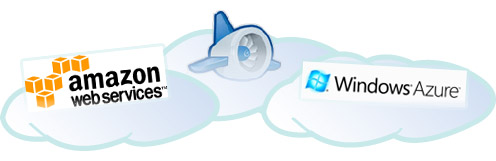
\includegraphics[width=0.8\textwidth]{./images/clouds.jpg}
\caption{AWS, GCP and Microsoft's Azure Services: the Cloud providers leaders} \label{fig:bigData}
\end{figure}


There are many cloud computing companies. Amazon and Google are two major players in this field, in which they offer Amazon Web Services (AWS) and Google Cloud Platform (GCP) cloud platforms, respectively. In order to have a more clear view of the actual Cloud landscape, we proceed to explain these two big cloud solutions, among some others in the following paragraphs.

\subsection{Amazon}
Since 2002, Amazon has been providing Cloud resources under the name Amazon Web Services \cite{amazon:aws}. AWS is a Cloud Computing Platform that offers scalable computing resources over the Internet. Amazon states that their users can have these resources up and running within minutes. AWS's offerings are accessed over HTTP, using REST and SOAP protocols. The communication with AWS is done through various web tools, browser plugins and standalone applications that provide an interface to AWS. Also this can be done using the Application Programming Interface (API) Amazon provides and integrating it into users' applications.

\bigskip
List of Amazon Web Services (related to this Thesis) \cite{amazon:aws}
\begin{enumerate}
\item Compute:
\begin{enumerate}
   \item Amazon Elastic Compute Cloud (EC2) is the Amazon IaaS solution. It provides scalable virtual machine based computation environments using the Xen Hypervisor \cite{Xen} to manage their Amazon Machine Image (AMI) instances. This server instances can be set up and booted within minutes, scaling their capacity according to computing requirements changes through a simple web interface. Amazon EC2 provides users with total control of their computing resources. 
   \item Amazon Elastic MapReduce (EMR) allows businesses, researchers, data analysts, and developers to easily and cheaply process vast amounts of data. It uses a hosted Hadoop framework running on the web-scale infrastructure of EC2 and Amazon S3.
\end{enumerate}
\item Storage  \& Content Delivery:
\begin{enumerate}
 \item Simple Storage Service (S3) provides Web Service based storage.
\item Amazon Glacier, Provides a very low cost long-term storage option (when compared to its S3 service). High redundancy and availability, but very long access latency. Ideal for archiving data.
\item AWS Storage Gateway is an iSCSI block storage virtual appliance with cloud-based backup.
\item Amazon Elastic Block Store (EBS) provides persistent block-level storage volumes for EC2.
\end{enumerate}
\item Database:
\begin{enumerate}
\item Amazon DynamoDB provides a scalable, low-latency NoSQL online Database Service backed by Solid State Disks (SSDs).
\item Amazon ElastiCache provides in-memory caching for web applications. This is Amazon's implementation of Memcached.
 \item Amazon Relational Database Service (RDS) provides a scalable database server with MySQL, Oracle, and SQL Server support.
 \item Amazon Redshift provides petabyte-scale data warehousing with column-based storage and multi-node compute.
\item Amazon SimpleDB, allows developers to run queries on structured data. It operates in concert with EC2 and S3 to provide "the core functionality of a database."
\end{enumerate}
\item Deployment
\begin{enumerate}
\item AWS Elastic Beanstalk provides quick and easy deployment and management of applications in AWS cloud. It is the main Amazon's PaaS solution. Elastic Beanstalk harnesses AWS services to complete its task successfully. Elastic Beanstalk takes care of the application's deployment: capacity provisioning, load balancing request, automatic scaling, etc. It supports Node.js, PHP, Python, Ruby, .NET and Java. 
\end{enumerate}
\end{enumerate}

Amazon Web Services is used by many cloud companies to provide new cloud services, including RightScale providing IaaS, Heroku providing PaaS or Dropbox providing SaaS.

\subsection{Google}

Google infrastructure has been built and continues being built to work on datacenters of commodity hardware as opposed to high-end hardware due to what is called the economy of scale: costs are reduced and overall computing power is maximized. Google has managed to develop a fault-tolerant elastically scalable system to work on several datacenters of commodity hardware, letting them to offer cheap Cloud Services.
\par
With that premise, Google entered the Cloud Computing business in 2008 with the Google App Engine offering. Whilst cloud provisioning is not their core business, they have given to the world numerous and important contributions in this field.
Google App Engine (GAE) is Google's PaaS solution. GAE allows users to host and run web applications and store data in Google-managed datacenters distributed around the world. It supports Java, Python, PHP and Google's Go programming languages. Users develop their applications on their local machines before uploading the applications to GAE. Then, it is GAE who takes care of the provisioning and deployment of the application uploaded on the infrastructure. Also automatic scaling is done during the life of the deployed application. Users do not need to keep an eye on the servers as this is GAE infrastructure's job. GAE software development toolkit (SDK) is provided by Google in order to allow users to develop their solutions in a simulated GAE's environment. Google also supplies APIs that can be used to integrate Google services with developer applications.
\par
On June 2012, Google announced Google Compute Engine (GCE) [cite] at Google IO. GCE is Google's IaaS solution. GCE allows users to run large-scale CPU works on Linux virtual machines hosted on Google's infrastructure. GCE provides all resources through the Google APIs Console, a collection of Google's APIs. GCE is very similar to Amazon's EC2 solution, both provides scalable CPU capacity. 
After that, Google unified its cloud solutions under the name of Google Cloud Platform (GCP) \cite{CloudGoogle}. 
\par
Google Apps \cite{GoogleApps} is the Google's SaaS implementation launched on 2006 and entirely based on Google's own infrastructure. It is a set of several Web applications which offer an online alternative to traditional offline office software. But Google Apps is not just an online office suite, but also a solution that allows users to communicate and collaborate between their projects easily. With Google Mail users can communicate with emails, online messaging and voice or video calls. Thanks to Google Docs users can create, edit, delete their documents, spreadsheets or slides. Google Calendar is a powerful online calendar application. Google Web Pages allows for publication Web pages. Google Drive offers file storage and synchronization to users. Recently, in the Google IO 2013 meeting, Google added to their Google Apps collection Google Hangouts. It creates online video meetings with a click, allowing users to work with clients or partners in real time.
\par
The main advantage of Google Apps is that everything is online, users do not need to install any software locally, they just need a computer with Internet connection and a Web browser to interact with Google Apps.

\subsection{Microsoft}

When analyzing this field, Microsoft has always something to offer. Windows Azure \cite{Azure} is Microsoft's platform for Cloud Computing. It was announced at the Professional Developers Conference in October 2008,  and commercially available since February 2010. In the beginning, Windows Azure supported only .NET development. However, now it supports many different programming languages, tools and systems, not only Microsoft-specific ones, but also third-party tools, such as Java, Ruby, PHP, Node.js and C++. Windows Azure is hosted in Microsoft-managed datacenters distributed around the world. Microsft states that Windows Azure enables users to deploy their applications within minutes and scale in/out them to any size in a fully automated way.
Windows Azure provides an API built on REST, HTTP, SOAP and XML that allows users to communicate with Windows Azure services easily. Microsoft also provides open-source Windows Azure client libraries for multiple programming languages. These SDKs help users build, deploy and manage their Windows Azure applications.
\par
Nowadays, Windows Azure Platform offers Infrastructure as a Service (IaaS) features that complement their initial offering of PaaS features. The Azure platform provides three distinct computing service models:
\begin{enumerate}
\item Windows Azure Web Sites, which is their PaaS service for Web hosting. Users can create web sites in PHP, .NET, Python and Node.js and deploy them using git, FTP or TFS. Web Sites supports horizontal scalability of web sites, from shared single instances to dedicated large instances.
\item Windows Azure Cloud Services, the traditional Microsoft PaaS service offering. Cloud Services are containers of hosted applications. Applications execute in virtual machines, also called instances, running Windows Server OS. Windows Azure itself manages the instances. Cloud Services allows to create scalable and reliable applications.
\item Windows Azure Virtual Machines, which comprises the Microsoft IaaS solution for their public cloud. Users create Virtual machines on demand. Unlike Windows Azure Cloud Services, users have total control of their created virtual machines. The Virtual machines offering includes Windows Server images as well as Linux distributions images provided by Microsoft partners.
\end{enumerate}

Windows cloud offerings are not just PaaS and IaaS solutions, but also SaaS tools. Windows Live is a Windows's SaaS which integrates search, email and a social network system. Skydrive is the cloud hosting Microsoft SaaS model. And Microsoft SharePoint is Microsoft collaborative cloud system, which allows multiple users to work together in real time.


\subsection{RackSpace}

Behind these three big players, RackSpace \cite{RackSpace} is one of the strongest cloud providers companies. Powered by an offering mostly based on the OpenStack Cloud Computing platform, Rackspace is a mostly open source based alternative to Amazon, Google and Windows Azure. One of its strengths is its ability to roll out the latest Openstack features, thus continuosly improving its functionality. Rackspace offers three different Cloud Services: Cloud Servers, their IaaS solution, Cloud Sites, which is their PaaS solution, and Cloud Files for storing files in the cloud, which is their SaaS solution. 
\par
As Eric Savitz states in Forbes article \footnote{Rackspace {S}lides {A}fter {H}ours {A}s {Q}4 {R}evs {M}iss {S}treet {V}iews - \url{http://www.forbes.com/sites/ericsavitz/2013/02/12/rackspace-slides-after-hours-as-q4-rev-miss-street-views/}}, in the last quarter of 2012, Rackspace total server amount has increased from 89.051 to 90.524, along with an increase of their total customers from 197.635 to 205.538.

\section{Behind the big Cloud providers}

Nowadays Amazon, Google, Microsoft are the biggest Cloud providers over the world, but this does not mean there are no other competitors offering excelent products in the Cloud field. Here we show the most promising cloud providers categorized by their offerings of resources: IaaS, PaaS and SaaS.

\subsection{IaaS}

Infrastructure as a Service cloud segment accounted for the majority of total market revenue in 2012 with more than half of the total public cloud market share \cite{aslett2013451}. The main responsibles for this impressive market quota are Google with its Google Cloud Platform, Amazon and Microsoft Azure, all of them deeply studied in the previous section 1.1. 


\subsection{PaaS}
Among the subcategories of Cloud Computing, the Paas layer is experiencing a fast growth. According to the Market Monitor research report \cite{aslett2013451}, PaaS accounted for the 24\% of the total public cloud revenue in 2012 and it is expected to grow between 2012 and 2016 at a 41\% compound annual growth rate (CAGR). Many companies are behind this success, in the following lines we describe some of them.
\par
Heroku \cite{heroku} is a cloud Platform as a Service (PaaS). It has been in development since 2007, what makes Heroku one of the original PaaS offerings in the world. Nowadays it is owned by Salesforce.com since 2008. At the beginning, Heroku supported only the Ruby programming language, but since then, Heroku has been adding support for more programming languages: Java, Scala, Python, Node.js, Clojure, Grails, Gradle, Play and PHP. Heroku platform is entirely based on the AWS EC2 and S3, giving it the ability to scale in/out to satisfy customers' demands.
According to former Heroku CEO Byron Sebastian, Heroku was hosting more than 1.5 millions applications by November 2010 \footnote{Heroku {B}oss: 1.5M apps, many not in {R}uby - \url{http://www.gigaom.com/2012/05/04/heroku-boss-1-5m-apps-many-not-in-ruby/}}.
\par
Openshift \cite{OpenShift} is another interesting and new cloud PaaS product offered and developed by Red Hat. OpenShift is free and open-source, although now it has a paid version which adds extra support and features. The software that runs the service is called OpenShift Origin \footnote{OpenShift Origin source code - \url{https://github.com/openshift}} and can be downloaded from Github, allowing users to change it according to their needs.OpenShift is aimed at Java, Python, PHP, Node.js, Perl and Ruby developers and, as many others PaaS, OpenShift is based on AWS, this one specifically in Amazon EC2.
\par
CloudBees \cite{CloudBees}
% \cite {http://www.infoworld.com/d/cloud-computing/which-freaking-paas-should-i-use-204189?page=0,2#paas2} %\cite{http://gigaom.com/2011/07/25/3-paas-lessons-from-cloudbees-funding/}
offers a Java-based PaaS to host, run and manage Java applications. It is one of the first PaaS aimed mainly at the Java developer. CloudBees supports any JVM-based programming language or framework. Jenkins Continous Integration (CI) tool is included in the CloudBees PaaS. It supports developers through the whole application life cycle directly in the cloud from Github. The CloudBees service provides middleware on top of some public cloud, such as Amazon Web Services, OpenStack and VMware vSphere though customers can also run the service on private cloud infrastructure.

\subsection{SaaS}
Software as a Service layer also strikes strongly in the Cloud race. SaaS represented 25\% of total cloud revenue in 2012 and it is expected to follow growing in the following years \cite{aslett2013451}. In the next paragraphs, we highlight two successful SaaS companies without forgetting Google SaaS products Google Apps and Windows SaaS offerings previously described.
\par
Talking about successful SaaS solutions, we always find Dropbox \cite{Dropbox}. Dropbox is a SaaS solution developed by Dropbox Inc., and launched on September 2008, that offers cloud storage and file synchronization to users. Dropbox uses Amazon S3 to store all files. 
In the released fact sheet of March 2012 \footnote{Dropbox {F}act {S}heet - \url{https://www.dropbox.com/static/docs/DropboxFactSheet.pdf}}, Dropbox stated that they had over 50 million users, and nine months later, in November 2012, Dropbox announced that they had over 100 million users \footnote{Dropbox {T}hanks a (hundred) million - \url{https://blog.dropbox.com/2012/11/thanks-a-hundred-million/}}.
\par
Another notable SaaS is Salesforce.com \cite{Salesforce.com}, which is one of the most popular SaaS Customer Relationship Management (CRM) platform. It offers on-demand CRM services for all kind of organizations. Salesforce.com presents two major products. Sales Cloud is a set of applications to manage sales, customers and other business activities more easily and efficiently; and Service Cloud, which provides organizations with a community help-desk.
\par
Unlike Dropbox or many other SaaS solutions, Salesforce.com is built on its own infrastructure: Force.com \cite{Force.com}, which is the Salesforce.com's PaaS product.


\section{Big Data}


Until now, we have showed the three most popular cloud paradigms: Infrastructure as a Service (IaaS), Platform as a Service (PaaS), and Software as a Service (SaaS) and how Google, Amazon, Microsoft and Rackspace among other companies offer their Cloud Services. Now it is time to move to one problem that has born with the outbreak of the Cloud Computing.
\par
Thanks to the features that Cloud Computing has brought with itself (pay-on-demand, elasticity, etc), lot of new applications have seen the light. Thanks to the new cloud business, they are now economically viable and before not. More and more novel applications harness the Cloud Computing paradigm every day, which means a never seen increase in the amount of generated as well as consumed data, called Big Data. Thus, scalable Database Management Systems (DBMS) have become a fundamental and critical part of cloud infrastructures \cite{agrawal2010big}.

\begin{figure}[htb]
\centering
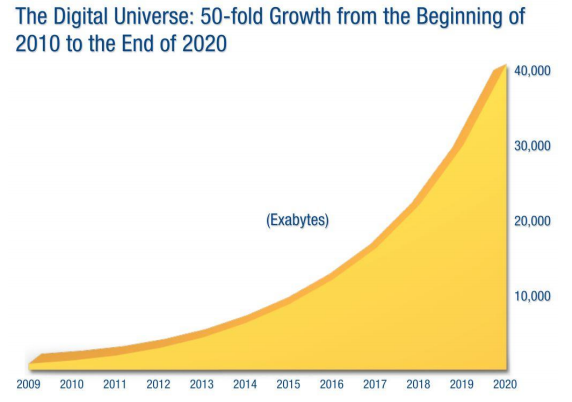
\includegraphics[width=0.8\textwidth]{./images/bigData.png}
\caption{Growth of data from the beginning of 2010 to 2020.} 
\label{fig:bigData}
\end{figure}

Figure 1.2 depicts how fast generated data is growing  \footnote{Figure extracted from IDC's Digital Universe Study, December 2012.}. International Data Corporation (IDC) estimates the digital universe will grow up to 40,000 exabytes, in more understandable words, 40 trillion gigabytes by 2020. From now until 2020, the generated data will double every two years \cite{gantz2012digital}.
\par
Google has been one of the first companies that has addressed the Big Data problem, which is handling large amounts of data. Google has designed its own MapReduce programming paradigm \cite{dean2008mapreduce}, allowing them to do scalable distributed batch processing of large amounts of data: Web request logs, crawled documents, etc. Related to this field, Google designed and implemented their own distributed file system to be used in combination with their MapReduce framework, which was called Google File System (GFS) \cite{ghemawat2003google}. These are systems designed to run on a large cluster of commodity machines and are highly scalable, but both implementations remain private to Google \footnote{Colossus is the new version of the GFS as mentioned in the Spanner paper on OSDI 2012 \cite{corbett2012spanner}}.
\par
After the publication of MapReduce and the GFS, Apache Hadoop \cite{ApacheHadoop} entered the scene as the open-source alternative to Google MapReduce and Google File System. Apache Hadoop is an Apache project that includes implementations of a distributed file system, namely Hadoop Distributed File System (HDFS)  \cite{white2012hadoop, shvachko2010hadoop}, and Hadoop MapReduce \cite{ApacheHadoop}, both inspired by Google projects. Hadoop was initially created in 2004 by Doug Cutting (and named after his son's toy elephant). In January 2008, Hadoop became a top-level Apache Software Foundation project. Nowadays it has many contributors, both academic and commercial (Yahoo being the largest commercial contributor), and continues growing.
\par
The field of distributed systems for Cloud Computing continued expanding, and as a logical next step, researchers needed a database for the applications to store the massive amount of data they were generating. Until then, the traditional and massive used Relational Databases Management Systems (RDBMS) have offered a simple and good solution according to the needs of the moment, but with the arrival of Web applications with massive numbers of users, the requirements of storage database systems for this new generation of applications have changed. Traditional databases did not offer a suitable and feasible storage solution to the new massive amount of data. In 2006, Google published a paper talking about BigTable \cite{chang2008bigtable}. Bigtable is a distributed storage system built on GFS for managing petabytes of structured data across thousands of commodity servers. Between its goals, we can find wide applicability, high performance, high scalability and high availability. To achieve such goals, BigTable uses a simple data model that supports dynamic control over data layout and format. Developers do not have to define a schema to store structured data, giving them a high flexibility when building applications. Albeit, such a simple data store brings with it a lack of characteristics. Lacking in particular are ACID transactions, Join operations and accessing through a natural query language like SQL that RDBMSes offer.
\par
As a response to BigTable we find Apache HBase \cite{ApacheHBase}, which is an open source project, modeled after Google's BigTable and written in Java. Developed as part of Apache Software Foundation's Apache Hadoop project, it became an Apache top-level project on 2010. Hbase uses HDFS as the underlying storage system for the created tables and the Apache ZooKeeper as a distributed coordination service, similar to the use of Chubby \cite{burrows2006chubby} in BigTable. Hbase features are similar to BigTable features; its implementation is very close to BigTable implementation with same properties. Main differences lie in implementation details. For example, how the memory is mapped or how the Garbage Collector works \cite {samar2011scalable}.
\par
HBase, BigTable and many others Cloud data stores are included in the group of so-called NoSQL databases \cite{NoSQLdatabases}. All of them are distributed storage systems mainly designed to offer a really good performance when dealing with Big Data, contrary to what traditional SQL databases do. 

\bigskip
\fixme{This thesis is structured as follows. In the next chapter, we present background knowdledge of ...... In chapter 3, we describe experiments....}
\bigskip




\chapter{Background}
\label{chapter:background} 


\section{Datastores:  From SQL to NoSQL systems}

A \textit{database} is an organized collection of data items, which are records of some real world information \cite{gray1993transaction}. Databases have always been extremely important in our society, from time ago with non-digital databases to nowadays with digital ones. They are a ubiquitous part of today's computing environment. 
\par
These database systems follow some data model, whose purpose is to determinate the logical structure of data items and how they are stored, organized and manipulated in data structures. As a vastly used data model we can found the relational model, used in SQL-based databases. 
\par
This data with its data model needs an structure to rely on, and this is called \textit{Database Management System} (DBMS). A DBMS is a suite of computer software programs that provides an interface between users and a database. They define mechanisms to build, store, maintain and modify one or more databases. 
DBMSes support any kind of applications, from business to Internet applications. They are one of the most important parts of many organizations and run critical applications that hospitals, airlines, banks and other types of organizations rely on for their daily operations.
\par
A relational database is a database which uses the relational model as its data model \cite{codd2001relational}. Its DBMS receives the name of Relational Database Management System (RDBMS) and it is the most popular example of database model. Most RDBMSes employ the SQL data definition and query language.
\par
Over the last three decades, RDMBSes have been the main technology for storing structured data. Even nowadays, the most popular DBMS continues being relational DBMS \cite{DBEnginesRanking}. RDMBS have been proved to be a good solution and have been evolved to fit new application requirements. These relational datastores have been and continue to be widely used. But with the amazing increase of generated data (Big Data), companies have seen how their needs have changed and they can not be addressed using the existing RDBMS technology, which have lead to the emergence of new datastores called NoSQL datastores, which are non-relational databases \cite{strauch2011nosql}.
\par
A NoSQL database is a database that uses less restricted data models than traditional relational databases, often loosing the ability to provide full ACID guarantees. Its main goals are its simplicity of design, horizontal scaling and higher availability. NoSQL systems are also revered to as "Not only SQL" due to some of them allow SQL-like query language.
\par
NoSQL is a term coined by Carlo Strozzi in 1998 to refer to an open-source relational database that did not use SQL \cite{Strozzi}. One year after, in 2009, the first NoSQL meet-up took placed in San Francisco. Computerworld magazine was there and stated in their article "No to SQL? Anti-database movement gains steam" that "NoSQLers came to share how they had overthrown the tyranny of slow, expensive relational databases in favor of more efficient and cheaper ways of managing data." \cite{ComputerworldNoSQL}. It evidents that new Web 2.0 Startups have started to use NoSQL datastores in order to handle the huge amounts of data the have to face instead the traditional RDBMS like MySQL \nocite{MySQL}, highly used in the startup environment before.
\par
In the last years, a great number of companies and projects have switched from relational towards non-relational datastores (NoSQL). By way of example, we find Cassandra \cite{ApacheCassandra}, developed at and used by Facebook, it is also used by Twitter \footnote{Cassandra at Twitter Today - \url{https://blog.twitter.com/2010/cassandra-twitter-today}} and Digg \footnote{Looking to the future with Cassandra - \url{http://about.digg.com/blog/looking-future-cassandra}}, Projet Voldemort developed and employed at LinkedIn \footnote{Project Voldemort: Scaling Simple Storage at LinkedIn - \url{http://blog.linkedin.com/2009/03/20/project-voldemort-scaling-simple-storage-at-linkedin/}}, or the cloud NoSQL datastore Amazon SimpleDB \footnote{Amazon SimpleDB -
\url{http://aws.amazon.com/simpledb/}} employed by Amazon.
\par
In order to realize how important the NoSQL environment is becoming , just a glance to the companies that are the pioneers or are in the cutting edge of the NoSQL movement is needed. They are enterprises running gigantic websites such as Google, Amazon, Twitter and Facebook, and others in the same field that use NoSQL datastores but modified to fit with their requirements due to their smaller scale.
\par



\subsection{The basic principles of NoSQL}
Three elements make up the basic pillars of the NoSQL datastores. They are the CAP theorem, the BASE theorem and the Consistency model. \cite{wang2012nosql}. These items are detailed in the following paragraphs.
\par
\begin{itemize}

\item CAP:
 In order to understand the design of NoSQL datastores, we must understand  the CAP theorem, introduced by Eric Brewer in 2000 \cite{CAP} and proved by Gilbert and Lynch \cite{ProbeCAP} in 2002. This theorem states that within a distributed data store, there are three properties that have a relationship of dependency, which are Consistency, Availability and Partition Tolerance.
\begin{itemize}
\item \textbf{Consistency} stands for clients must see always the same data.
\item \textbf{Availability} means each read or write request receives a response whether it was successful or failed.
\item \textbf{Partition Tolerance} means everything works despite physical networks partitions, except in case of total network failure. A network is partitioned when message losses occur between any two nodes of the system.
\end{itemize}

The CAP theorem affirms that a distributed data store can only satisfy at most two of these three conditions. Indeed, distributed systems like Cloud datastores, must allow Partition tolerance, otherwise they would be non-distributed systems. Therefore, this leaves us with only two real options to choose from: Consistency and Availability. Figure 2.1 depicts the CAP theorem's affirmation, only two out of the three properties share a segment, so that only two of them can be chosen at once.

\begin{figure}[htb]
\centering
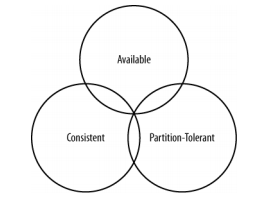
\includegraphics[width=0.5\textwidth]{./images/CAP.png}
\caption{The CAP theorem.} \label{fig:CAP}
\end{figure}

\par
According to this theorem, there are three possible views to design datastores, they are CA (primarily support Consistency and Availability), AP (primarily support Availability and Partition tolerance) and CP (primarily support Consistency and Partition tolerance).
\par
Figure 2.2 shows a graphical description of where each of the most relevant NoSQL and SQL solutions fit on the CAP continuum. The graphic was inspired by Dwight Merriman, CEO and founder of MongoDB, and updated by Eben Hewitt, Apache Cassandra Project Chair.
\begin{figure}[htb]
\centering
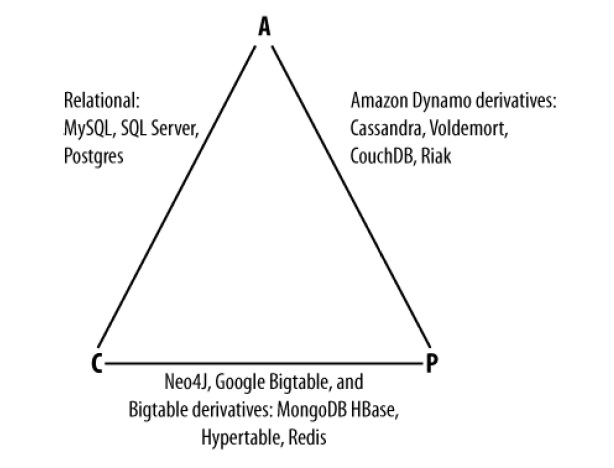
\includegraphics[width=0.6\textwidth]{./images/cap-examples.png}
\caption{CA, CP, AP real solutions.} \label{fig:CAP-examples}
\end{figure}

\par
As a brief summary, we can settle that traditional RDBMSes take Consistency and Availability but not Partition Tolerance. On the other hand, these new Cloud datastores, such as BigTable or Amazon Dynamo, take Partition Tolerance as we stated before, throwing away either Availability or Consistency respectively. 

\item BASE: 
ACID (Atomicity, Consistency, Isolation and Durability) datastores (traditional RDBMSes) are less powerful for distributed systems as they focus on strong consistency for transactions setting aside availability. Thus, it brings up a new softer consistency model widely adopted between most of the NoSQL datastores, which is: BASE \cite{pritchett2008base}, an acronym for Basically Available Soft-state services with Eventual-consistency. Basically available means partition failed could be supported, soft state indicates that the system could be non-synchronous sometimes and eventual-consistent implies that the data should be consistent after a reasonable time span. BASE can be seen as the opposite to ACID, while ACID requires the strongest consistency, BASE accepts eventually consistency, achieves availability and leads to levels of scalability that can not be obtained by any other way.

%\fixme{figura del marcador de firefox, el qe sale ejes x e y, y como acid o base y manchas verdes.}

\item Consistency:
\textit{Consistency} is a datastore feature that has brought lot of controversy. As we have stated before, in the domain of Cloud datastores, trade-offs between consistency and availability (also referred to as latency in new CAP studies \cite{abadi2012consistency}) have been studied and done \cite{brewer2012cap} \cite{gilbert2012perspectives}. Consistency is divided in two sides: the client-side and the server-side. Client-side consistency refers to how and when users see updates made to an object in the storage system. There are three types, which are \cite{vogels2009eventually}:
\begin{itemize}
 \item \textbf{Strong consistency}, which means reading always returns the most recent written value.
\item \textbf{Eventual consistency}, which essentially means that all updates will propagate through-out all of the replicas in a distributed system, but this may take some time. Thus, all replicas will eventually converge to the same value, achieving strict consistency. 
\item \textbf{Weak consistency}, which stands for zero guarantees that subsequent access will return the updated value. The term \textit{inconsistency window} is used to refer to the period between the update and the moment when any user will see the updated value.
\end{itemize}

There are lots of eventual consistency levels \cite{wiki:consistency}, but they are out of the scope of this study.
\par
On the server side, consistency refers to how updates are done through the system and what guarantees the system gives with respect to updates. Here the consistency level can be modified, it can be tweaked from weak/eventual to strong consistency by playing with the number of replicas of the data that are contacted \cite{vogels2009eventually}.
\par
This "no total consistency" term has caused some uproar in the industry because as they argue, data is the heart of their business. But then why most popular web applications such as Amazon, Facebook or Twitter are using it. It is because companies have to choose between giving clients their results within a decent response time, or wait tons of minutes to get perfect consistent data. Nevertheless, it is worth mentioning that not all NoSQL datastores throw away consistency following strictly the scope of the BASE model, as we have explained, some NoSQL solutions offer degrees of consistency or even total by doing some trade-offs \cite{chang2008bigtable} \cite{cooper2008pnuts} \cite{ApacheHBase}.
\par
As an example, BigTable and HBase are strongly consistent (althought not fully ACID compliant) while Cassandra meets the eventual consistency and offers degrees of it.
\end{itemize}

After understanding the basic principles of NoSQL solutions, now we show the common key features these systems present.

\subsection{Key features of NoSQL Datastores}

Besides the three explained NoSQL pillars, Rick Cattell states in a 2010 SIGMOD paper \cite{cattell2011scalable} that NoSQL systems generally have six key features:
\begin{itemize}
\item The ability to horizontally scale "simple operation" throughput over many servers. ("simple operations" stands for key lookups, reads and writes of one or small number of records). In NoSQL datastores, query operations are simpler and easier than relational Joins or other complex SQL queries.

\item The ability to replicate and to partition data across servers based on a shared-nothing approach.

\item Clear and understandable interface to communicate with rather than SQL binding as in most relational databases.

\item Do not support ACID transactions in contrast to most relational databases. Instead they offer BASE (Basically, Available, Soft state, Eventually consistent), a softer concurrency model.

\item Efficient use of distributed indexes and RAM for data storage

\item Schemaless, which means users can add new attributes to data records at any time.

\end{itemize}


\subsection{Types of NoSQL Datastores}

Many of the organizations that have adopted NoSQL solutions to support their projects deal with massive amounts of unstructured or semi-structured data that does not fit anymore with the traditional fixed SQL data models. Each commented type of data features different characteristics, whereby each one requires different approaches to tackle it, which has turned out in different types of NoSQL solutions.
\par
According to the approach outlined by Rabi Prasad Padhy in a 2011 International Journal of Advanced Engineering Sciences and Technologies (IJAEST) paper \cite{padhy2011rdbms}, on a basic level, there are three main types of NoSQL datastores according to their data model:
\begin{itemize}
\item Key/value stores: Data is stored as key-value pairs; key is used as an index to find its value. These datastores can hold structured and unstructured data. Query operations are limited as the internal structure of data is not known. Some examples are Amazon's SimpleDB, Riak, Redis, Azure, GT.m, MemcachedDB and Voldemort.
\item Column-oriented Databases: Instead of sets of data in a structured table of columns and rows as in relational databases, Column-oriented databases contain one extendable column of related data. Examples of ColumnFamily databases are Google BigTable, Cassandra, HBase, HyperTable and OpenNeptune.
\item Document-based stores: Systems store indexed documents, as just defined. Documents hold data in a standard format such as JavaScript Object Notation (JSON). Users can add whatever they need to a document. The elements of a document can be arbitrarily complex and can be queried. Document databases are Apache CouchDB, MongoDB and Raven.
\end{itemize}




 
\chapter{Technical background}
\label{chapter:technical background} 

In the following section we focus on the Column-oriented datastores, explained before, and in particular in the HBase solution, one of the most popular and open-source Column-oriented datastores.

\section{Column-Oriented Datastores}

When referring to Column-Oriented datastores, also called Extensible Record Stores, Bigtable is the pioneer. Bigtable and many other datastores of this type present a simple and flexible data model that can be extended at any moment.
Some famous Column-Oriented datastores are Apache HBase \cite{ApacheHBase}, HyperTable \cite{HyperTable}, Apache Accumulo \cite{ApacheAccumulo}, and Apache Cassandra \cite{ApacheCassandra} between many others.
\par
Among all these solutions, HBase \cite{george2011hbase} is likely the most popular open-source Column-Oriented datastore and is the one that we are going to use for our experiments.
\par
In the next section, we will describe HBase and how it works in order to fully understand this thesis.


\section{HBase}


HBase is an important Apache Hadoop-based project, which, as we stated before, is modeled on Google's BigTable database. Hbase can be characterized as a distributed, fault tolerant scalable database built on top of the HDFS file system. It belongs to the group of column-oriented datastores and uses Zookeeper for management of partial failures.
\par
Below, all must-known aspects of HBase are presented: HBase data model, storage, architecture, write/read/delete paths and the client API.


\subsection{Data Model}

HBase stores data items, those are key/value pairs. The keys are multidimensional. Each single value is indexed by a row key, column key and a timestamp \footnote{Timestamp, also known as version number}. Row keys are unique and allow the user to address all columns in one logical row. The column key is the combination of a column family and a column qualifier. Column families are the main unit of separation within a table. The last part is the timestamp which is used for versioning the data. Timestamp is usually automatically generated by the corresponding Region Server but it can be specified by the user.
\par
Summarizing, a key is commonly represented as the tuple (row, column, timestamp), which addresses a specified value:

\bigskip

			\centerline{\textbf{(row, column, timestamp) -\textgreater value}}
\bigskip 

where column equals (column family, column qualifier), timestamp is a 64-bit integer and row, column family, column qualifier and value are uninterpreted array strings, since in HBase everything is store as bytes.

\begin{table}[htbp]
\begin{center}
\begin{tabular}{|l|l|l|l|}
\hline
\textbf{Row Key} & \textbf{Time Stamp} & \textbf{Family:Qualifier} & \textbf{Family:Qualifier} \\ \hline
"com.cnn" & t9 &   & anchor:cnnsi = "Y" \\ \hline
"com.cnn" & t8 &   & anchor:look = "X" \\ \hline
"com.cnn" & t6 & contents:html = "" &   \\ \cline{1-2}
"com.cnn" & t5 & contents:html = "" &   \\ \cline{1-2}
"com.cnn" & t3 & contents:html = "" &   \\ \hline
\end{tabular}
\caption{Example Hbase table given by \cite{ApacheHBaseDataModel}}
\end{center}
\end{table}

A cell is a set of data items with a common row and column key (remember that column key stands for (column family:column qualifier)), being the cell key = (row,column). Each data item in a cell is called a version of that cell.
\par
HBase supports multiversion of cells. Each version of a cell is stored as a separated cell, next to others versions of that cell. Versions of a cell are sorted descending by the timestamp so that users will see the newest value first while reading it.
Another HBase table feature is that it does not store NULL values as RDBMSs do. Files storing the data only contain data explicitly set.
\par
A table is organized by grouping cells into rows. These cells are sorted lexicographically by row key first and then by column key, so row keys lexicographically close will be stored near to each other. The sorting allows the table to be partitioned into the denominated \textit{regions}, which hold exclusive ranges of row keys. The regions of a table are distributed between different nodes.

\subsection {Storage}

The real view of tables differs from the conceptual view explained before. Physically, tables are stored on a per-column family basis, which means that all column family members are stored together in files called HFiles/StoreFiles. Such a thing brings an advantage, which is that they can be compressed together. Column families must be declared while creating the table, whereas column qualifiers can be added to column families at any time.
\par
As written before, the HBase storage files are called HFiles. They are based on Hadoop's TFile \cite{TFile} class and mimic the SSTable format used in Google's Bigtable system. What is stored inside them is called KeyValue instances. They are the physical view of the conceptual cells. The whole cell, with its structured data (row length, key type, etc.) is what is a KeyValue object. Figure 3.1 shows a conceptual depiction of the KeyValue format.
\par

\begin{figure}[htb]
\centering
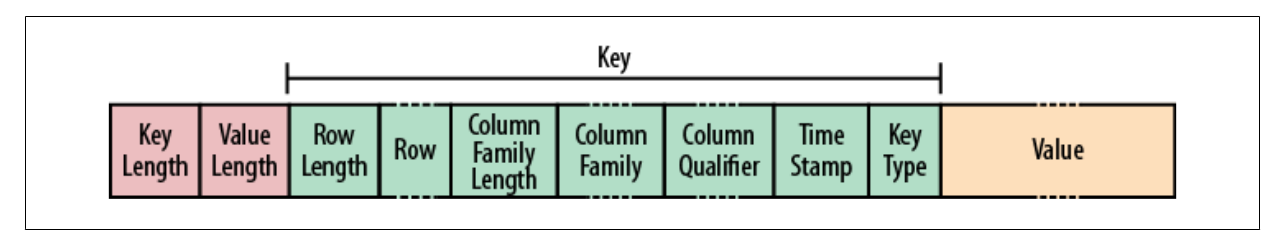
\includegraphics[width=0.8\textwidth]{./images/keyvalue.png}
\caption{The KeyValue format, extracted from HBase: The definitive guide \cite{george2011hbase}.} \label{fig:keyvalue}
\end{figure}


\subsection{Architecture}

HBase consists of three layers: the client, the server and the storage layers. The server layer consists of a master server and many region servers; the client has the library to communicate with the existing HBase installation; the storage layer is composed of a file system and a coordination service. Hadoop Distributed File System (HDFS) is the most used and tested file system to work with HBase. As the coordination service, ZooKeeper is the one HBase uses for its distributed coordination service. In the following section each component is explained as well as some HBase's features.

\begin{figure}[htb]
\centering
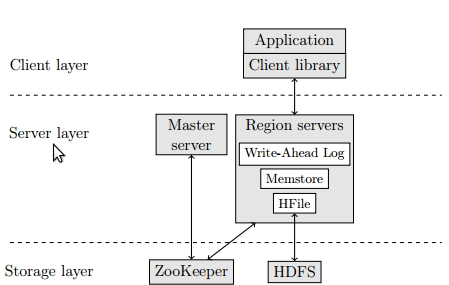
\includegraphics[width=0.8\textwidth]{./images/HBaseLayers.jpg}
\caption{HBase architecture overview} \label{fig:hbaselayers}
\end{figure}


\subsubsection{Storage layer}

The storage layer is composed of a chosen file system for the HBase cluster and a coordination service:

\begin{itemize}
\item File system: HDFS \cite{ApacheHadoop, HDFSarchitecture} is the default file system when deploying an HBase cluster, but optionally it can be replaced by any other file system. For HBase, HDFS is the primary option as it is scalable, fail safe, has automatic replication and is built to run on a set of commodity hardware. It fits with the needs of a distributed system. 

% Hadoop MapReduce is always used with HDFS as the underlying file system, thereby HDFS performance when dealing % with a huge amount of data, as Hadoop MapReduce does, is optimized. 

\item Coordination service: Apache ZooKeeper \cite{ApacheZooKeeper, hunt2010zookeeper, junqueira2011zab} is an open source project and a part of the Apache Software Foundation. ZooKeeper is a highly-reliable distributed coordination service, comparable to Chubby \cite{burrows2006chubby}, owned by Google and used for BigTable. Its aim is to offer a file-system-like access to clients with directories and files (znodes) that are used to store data, register services or watch for updates in a simple interface. In HBase, every region server creates a node in ZooKeeper, which will be used by the master to discover them. HBase uses ZooKeeper to choose the unique master and to store "-ROOT-"'s address too.
Master server and region servers communicate with ZooKeeper to keep track of the current situation of the regions and region servers.
\end{itemize}
\subsubsection{Server layer}
Server layer is compound of two parts:
\begin{itemize}
\item Master: The master server does not store any actual data and is not part of the retrieval path. It is responsible for assigning regions to region servers, handling load balancing of regions across region servers, unloading busy servers and moving regions to servers that are freer, and performing garbage collection of files. Since it never stores or provides data to clients or region servers, is slightly loaded. Further, it takes care of all administrative operations such as schema changes or creation of tables or column families.
\par
If the master server goes down, the cluster can still work as the HBase client does not talk with it directly. Nevertheless, master should be restart as soon as possible.
\item Region: As Lars George states in his book HBase: The definitive guide \cite{george2011hbase}, a \textit{region} is the basic unit of scalability and load balancing in HBase and is responsible for storing the actual data. Inside it, we can see contiguous ranges of rows stored together. Clients communicate directly with region servers to run all retrieve / write data operations. Each region is served by only one region server, although those ones can store multiple regions. These region servers also split regions into two pieces at the row key which is in the middle of the whole region once they have exceeded the maximum region size.
\end{itemize}

\subsubsection{Client layer}

Client needs to be able to find the region server which has a specific key. In order to achieve that, client communicates with the Zookeeper server and then retrieves the location of a table called "-ROOT-" table from there. This table stores information about all regions in the ".META." table, which is another table storing where regions are and its row key ranges. So client reads the ".META." table and receives the exact address of the correct region handling a determined key or key range. Thanks to this three level lookup, client is able to find the correct region server and perform his operations. For optimizing the process, client caches region locations because once the user table region is known, it can be accessed straightforwardly without the three level lookup.


\subsection {Write}
This subsection clarifies how writes and related stuff are done in a such a complex system as HBase is.
\par
Write requests are hold by Region Servers. Those components have three main elements: Write-Ahead Log (WAL), Memstore and HFiles. The WAL acts as a log for all modifications done to data in that exactly region, guaranteeing atomicity and durability. The WAL allows regions to recover from server failures. It contains all previous modifications and can be used to replay the data, achieving the last known stable stage. Memstore is an in-memory buffer that contains recently updated data items sorted by key. It works similar to how caches work on microprocessors, MemStore caches data items, thus reducing read and write latencies. There is one MemStore for each column family of a table in the region. HFiles stores actual HBase's data.
\par
HBase stores data to disk similar to how a Log-Structured Merge Tree works \cite{o1996log}. First, when new data arrives at the region server it is put on the Write-Ahead Log (WAL). If the write to the WAL is achieved, the region server writes the data into the memory store. Region continues writing data to the Memstore until a configured maximum size. Once that threshold is reached, Memstore flushes the data to disk. When flushing, multiple HFiles are created, one per column family, which affects negatively to HBase's performance. Massive amount of tiny files stands for more seeks and thus, higher latencies while reading. Due to that, HBase monitors the number and size of these files and does compactions from time to time. A compaction is the process of merging multiple HFiles together, there are two types:
\begin{itemize}
\item Minor compaction: It is responsible for rewriting the last few files into a larger one. It is triggered when certain properties and ratios are reached.
\item Major compaction: It merges all files of a region into one single file. It is usually triggered every twenty-four hours or even more due to its heavy load. Sometimes, it is recommended to disable major compactions and manage them manually as they rewrite all files.
\end{itemize}

HFile files store an index at the end of the file to locate blocks. The index is loaded into memory when the HFile is opened allowing look-ups to be performed with a single disk seek. For a more complete overview of how these files are designed refer to \cite{white2012hadoop}.

\subsection{Read}
Next paragraph explains reads in HBase.
\par
First of all, when a Region Server receives a Get request, it checks if the desired row is in the MemStore. If not, it starts to search through the HFiles starting from the newest working towards older HFiles, which means to take a look through the disk contents because the data could be spread over multiple files.

\subsection{Delete}
Here we explain how data is deleted from a HBase cluster. We must have clear that rows are never directly erased from HBase. When a Region Server receives a Delete request, it looks for the row and writes a delete marker to it. Whenever a Get request tries to access a row that has been previously deleted, it will find the delete marker and will not be returned. During the next major compaction, rows with the delete marker will finally be deleted.

\subsection {HBase API}

HBase provides a powerful client API written in Java as HBase does. It provides from basic operations to expensive ones. The initial set of basic operations are called CRUD operations which stands for "Create, Read, Update and Delete".

\bigskip


\textbf{Definition 1. }Put 

There are two groups of Put operations, first one works on single rows and the other works on a list of rows, both allow users to store data into HBase's tables in a transparently manner. Defined as:
\par
\bigskip
\centerline{\textit{put([List]Put put[s])}}
\bigskip

The user needs to supply a Put object or a list of them. ThesePut objects are created with the Put constructor:
\par
\bigskip
\centerline{\textit{Put(byte[] row)}}
\bigskip
A row key is supplied in order to create the Put instance, and once the user has created it, he/she can start to add values to the specified Put instance with the \textit{Put.add(value)} method. The user can also supply a version number for a given key/value pair (timestamp), but if it is not specified, HBase gives to it a version number created from the current time of the Region Server responsible for that given row.
\par
When providing the value for the \textit{Put.add()} method, as opposed to what happens with column qualifiers that can be whatever the user needs, an existing column family need to be given. Column families are usually defined when creating tables, but the user can always add new families calling to an expensive operation. It is because of that, HBase heavily recommends users to use fixed column families, although they can be altered.
Unlike column families, new column qualifiers, version numbers and row keys can be provided on-the-fly within Put operations with no extra cost.
\par
The HBase API allows to use a built-in client-side write buffer that collects sets of Put operations before sending them as a unique RPC connection to the corresponding server. Hence, less RPC connections are needed resulting in an increase of the overall performance. HBase is smart enough to group and sort Puts by Region Server. If write buffer is not used,  any time a Put operation is completed, HBase's API will submit it to the right Region Server.

\bigskip
\textbf{Definition 2. }Atomic Compare-and-Set

As a variation to the Put calls, the user can use Check and Put operation, defined as:
\par
\bigskip
\centerline{\textit{checkAndPut(byte[] row, byte[] family, byte[] qualifier,byte[] value, Put put)}}
\bigskip
This method allows users to issue Puts with a checking point. Only if the check step is successfully completed, the put operation is performed, everything as an atomic operation. It is really useful when dealing with data that needs previous values or similar stuff.
\par
All rows inside the Put object must be equal to the given row. The user can not use this operation to check different row keys. Otherwise, Check and Put operation will fail.

\bigskip
\textbf{Definition 3.} Get

Like in HBase Put method, there are two groups of Get operations, the ones that work on a single row and the others that operate with multiple rows. Both allows the user to retrieve data stored in HBase's tables.
\par
Get operation is defined as:
\par
\bigskip
\centerline{\textit{get([List]Get get[s])}}
\bigskip
The user needs to supply a Get object. These objects are created with the Get constructor like in Put operations. it is:
\par
\bigskip
\centerline{\textit{Get(byte[] row)}}
\bigskip
In analogy with Put constructor, the user provides a row key to the Get method in order to get a Get instance. Get operation is bounded to a specified row, but can retrieve any data stored in it, from one value to all columns with its values.
\par
The user can add parameters to the Get object in order to narrow down the search. They will act as filters. If the user wants everything of a row, no filters are used, but if the user only wants a column family, the \textit{Get.addFamily()} method must be used. Same thing happens if the user only wants a column qualifier from a column family (\textit{Get.addColumn()}), or the row with a known timestamp (\textit{Get.setTimeStamp()}).
Lastly, there are methods, acting as filters, that allow users to specify how many versions want to be retrieved (\textit{Get.setMaxVersions()}) and many others.
\par
Like in Put method, the user can retrieve a list of Gets, instead of only one row. The main difference is that the user issues a list of Gets, instead of one Get object. The result will be an array of Results, one for each Get instance.

\bigskip
\textbf{Definition 4. }Delete

HBase client API provides a method to delete data from its tables. Delete method is defined as:

\par
\bigskip
\centerline{\textit{delete([List]Delete delete[s])}}
\bigskip
Once more, the user is able to delete one row by one row or a list of them, the difference is the type of parameter: a Delete instance or a list of them.
\par
As with Get and Put calls, the user has to create a Delete instance and then adds details (filters) about the data he/she wants to remove, the constructor is:

\par
\bigskip
\centerline{\textit{Delete(byte[] row)}}
\bigskip

A row is provided. Subsequently, what user wants to be removed is added to it using different methods. Most important ones are \textit{Delete.deleteFamily()} method, used to remove an entire column family, including all its columns, and \textit{Delete.deleteColumns()} method, which operates on one column of a given column family, deleting all versions contained or just the cells matching the timestamp if it is provided. There are other types of Delete methods, but less used.

\bigskip
\textbf{Definition 5. }Atomic Compare-and-delete

As a variation to the Delete call, the user can use Check and Delete operation. It is defined as:

\par
\bigskip
\centerline{\textit{checkAndDelete(byte[] row, byte[] family, byte[] qualifier, byte[] value, Delete delete)}}
\bigskip

It works as a Delete operation but adding a previous step in which a specify row key, column family, column qualifier and value are checked before deleting the desired row.
\par
Users can only check and delete on the same row. If the row key differs from the one pointed by the Delete instance, the CheckandDelete operation will fail.

\par
\textbf{Useful hint. }Row Locks for Row mutations:

Previous operations: Put, Delete and CheckAndDelete are executed in such a way that they guarantee row level atomicity. They are executed entirely. A row lock is provided by the corresponding Region Server, protecting the row from other users trying to access it. Not from users trying to read it, only for those submitting row mutations operations.

\bigskip
\textbf{Definition 6. }Scans

Scan operation allows the user to scan a range of data, from one row to a determinate stop row, taking advantage of the underlying sequential storage layout HBase has. The scan returns every row between the chosen range of rows. This operation is not executed atomically, it can be partially executed. Hence, returned data can be outdated if there has been a write operation during the scan. 
\par
Scan operation is really similar to Get method and it works as a iterator, it means that user has a Scan instance and he/she must iterate over it to get all the results.
\par
Scan method is defined as:
\par
\bigskip
\centerline{\textit{getScanner(Scan scan)}}
\centerline{\textit{getScanner(byte[] family)}}
\centerline{\textit{getScanner(byte[] family, byte[] qualifier)}}
\bigskip
Each of them narrow the read data, from a general Scan to one that only returns values from a Column Family and inside it, from a Column Qualifier.
\par
As in Put or Get methods, Scan object is created with its constructor, which is:
\par
\bigskip
\centerline{\textit{Scan(byte[] startRow, byte[] stopRow)}}
\bigskip

It returns a Scan instance. Start row is mandatory and always inclusive, while stop row is not and is exclusive ( [startRow, stopRow) ). The user can submit filters as well.
\par
Once the user has created the Scan instance, the user can narrow the scanned data using \textit{Scan.addFamily()} method or even a more restricted  one which is, \textit{Scan.addColumn()}. There are more mechanisms that allows users to set timestamps or time ranges.
\par
It is important to notice that the Scan operation do not cover all results within a single RPC connection, but instead it returns row by row since they can be very large. In order to iterate over the results, Scan presents \textit{next()} and \textit{next(int nbRows)} methods. Using them, each call will be traduce to a RPC for every row.
\par
Summarizing, HBase Scan method can be seen as  a lot of Gets operations, and indeed, it is what it does.


\subsection{HBase properties}

In this section we discuss the CAP theorem and the BASE and the ACID model for HBase. 
\par
HBase is called a CP type system since it supports Consistency and Partition Tolerance facets of the CAP model.
HBase offers Partition Tolerance as it survives message loss due to server failures, network problems, etc. If a region server collapses, other nodes take over the tasks which comprised the region by replaying its commit log and memstores.
Regarding consistency, HBase does trade some availability to achieve a stronger level of consistency. After a write completes, the next read will see the lastest value because at any given time only one region server is responsible for that key.
Availability is given up because if a region server dies, its data will be unavailable until another region server comes up and picks up the died regions.
\par
HBase is not an ACID compliant database, but it guarantees some ACID properties, such as atomicity within a single row but not across multiple rows, or strong consistency thanks to the design of regions only being hosted in one region server at any one time, which creates only one responsible for serving a given data and also thanks to the Multi-Version Concurrency Control (MVCC) \footnote{MVCC \cite{bernstein1983multiversion} is a solution that keeps a list of versions of each data item. From the point of view of the user, he or she will only see one data item, but from the system side, each update of the data item will correspond to a newer version number of the same data item. Thus there will be multiple versions stored, but only one is the lastest.} used by HBase to manage concurrent access to the database (no locks are used as in old ACID SQL databases, instead timestamps \footnote{Timestamps, also called version numbers, are the MVCC data structures} offers all HBase needs to get all of ACID).



\section{HDFS}
%un poco de introduccion aqui
HDFS is the distributed file system of the Apache Hadoop open-source framework that provides high-throughput access to the stored data. It is scalable, fail safe, offers automatic replication and is built to run on a set of commodity hardware.
\par
HDFS consists of a master node called NameNode, and slave nodes called DataNodes. HDFS splits the data into equal size blocks and spread them across all available DataNodes in the cluster. Each block is replicated three times by default with at least one replica within the same node. The NameNode retains all metadata about blocks and replicas.

\begin{figure}[htb]
\centering
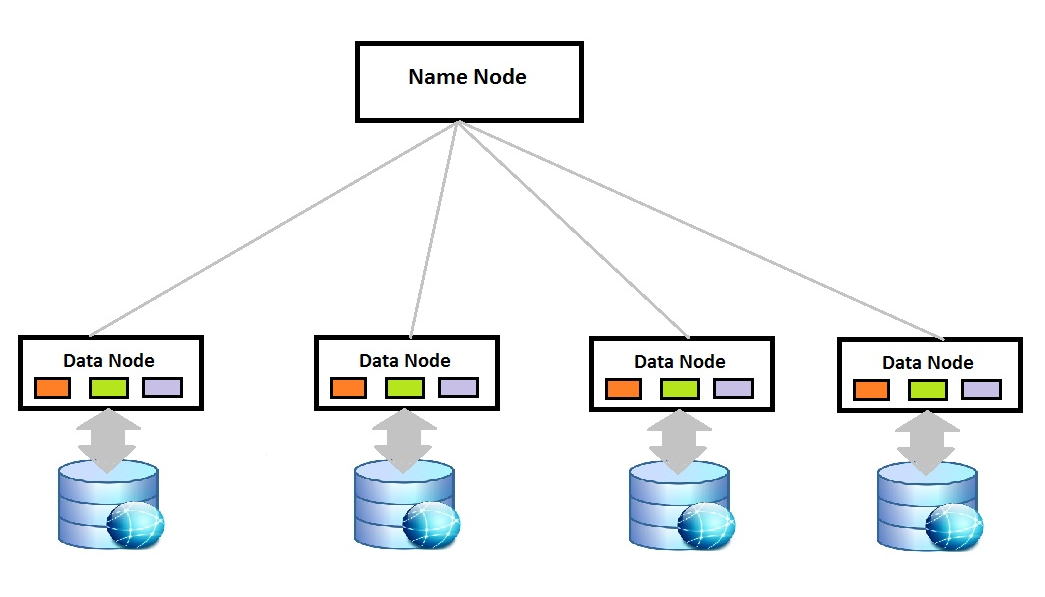
\includegraphics[width=0.8\textwidth]{./images/hdfs.png}
\caption{HDFS overview} \label{fig:hdfs}
\end{figure}


\section{MapReduce}

MapReduce programming model allows to abstract from the complexity of writing concurrent programs. It is based on two functions: map() and reduce(). The framework takes care of invoking them in the correct order on the input data and scheduling parallel execution of these two functions across any number of computation nodes. The user just needs to write the map and the reduce functions.
\par
Map takes an input as key/value pair (\textless k1, v1\textgreater), and emits a number of intermediate key/value pairs as its output (\textless k2, v2\textgreater). The MapReduce job group together all the values which have the same intermediate key and passes them to the Reduce function (\textless k2, list(v2)\textgreater).
\par
Reduce accepts intermediate key and a set of values for that key as input(\textless k2, list(v2)\textgreater). For each pair the reduce function outputs a final key/value pair (\textless k2, v3\textgreater). Map and reduce functions can be summarized in the following equations:

\centerline{map(\textless k1, v1\textgreater) \:\:  -\textgreater \:\:   list(\textless k2, v2\textgreater)}
\par
\centerline{reduce(\textless k2, list(v2)\textgreater) \:\:  -\textgreater \:\:  \textless k2, v3\textgreater}

\bigskip
\par

The MapReduce model fits with many large-scale data problems and can be efficiently implemented to support problems which input data is hundreds or thousands of megabytes. Due to the large size of the data, is more efficient and easier to move the computation instead the data. Therefore, in a MapReduce framework, data is splitted into blocks and distributed accross many nodes in a cluster. Then, it is the MapReduce framework who takes advantage of data locality by moving computation to data rather than sending data to the nodes. That is, MapReduce schedules Map tasks close to the data block on which they will work, so it can be read and processed very fast for each node in parallel. This is the prinpicipal factor in MapReduce's performance.

\subsection{Hadoop MapReduce}

% for a more non-technical view, go to the introduction 1.

Hadoop MapReduce \cite{ApacheHadoop} \cite{white2012hadoop} is the popular Apache open-source Java implementation of the MapReduce model. It is always used with HDFS as the underlying file system. Hadoop MapReduce consists of a single master node called JobTracker and worker nodes called TaskTrackers. When using HDFS with Hadoop MapReduce, TaskTrackers live on the same nodes where HDFS DataNodes live.
\par
When a Hadoop MapReduce is submitted, it is divided into map tasks, also known as mappers, and reduce tasks, also called reducers. Each task is executed on a available slot in a worker node. Each worker can handle a fixed number of either mappers or reducers.
\par
The number of mappers is determined by the number of data blocks as each map task processes a block of input data. Each data block should be as close to the map task as possible, so data locality can be exploited and the amount of IO reduced. On the other hand, the number of reduce tasks is specified by the application.

\begin{figure}[htb]
\centering
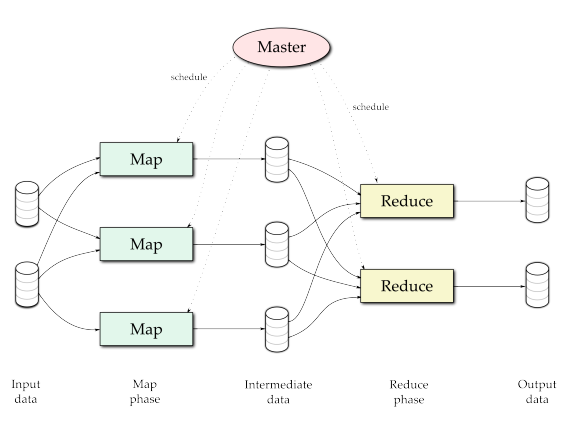
\includegraphics[width=0.8\textwidth]{./images/mapReduceModel.png}
\caption{MapReduce workflow} \label{fig:mapreducemodel}
\end{figure}


Mappers start processing its associated data block and emit key/value pairs. Each mapper output is allocated to a particular reducer by the application's partition function; pairs with the same key are sent to the same reducer. Between the map and reducer stages, the intermediate data is shuffled in order to move it from map nodes to its reduce nodes. This shuffle phase is started as soon as mappers produce pairs. After all mappers finnish and shuffle phase completes, reducers move into the reduce phase, where the reduce function is applied to the intermediate data and the final output is written.
\par







\chapter{Environment}
\label{chapter:environment}

Here we describe the environment we work in. We describe the cluster used for testing, the software deployed and the dataset of our experiments.

\section{Triton}

For this final project we have been using Triton for testing solutions as well as doing performance evaluation tests. Triton is a high performance cluster owned by Aalto University School of Science and used by its members \cite(wiki de triton).

As of July 2013, Triton has 238 compute nodes divided in 5 big groups:

\begin{enumerate}
\item Frontend node: HP SL390s G7 with 48GB of memory. The login node through which rest of the cluster is accessible to users.
\item 109 compute nodes HP ProLiant BL465c G6, each equipped with 2x Six-Core AMD Opteron 2435 2.6GHz processors. 80 compute nodes cn[01-80] have 32GB (cn[65-67] used for NFS servers needs), 32 others have 64GB cn[81-112], 4xDDR Infiniband port and local SATA drive with diskspace available ~215GB.
\item 118 compute nodes cn[113-224], tb[003-008] are HP SL390s G7, each equiped with 2x Intel Xeon X5650 2.67GHz (Westmere six-core each). Every SL390s G7 node has 48 GB of DDR3-1066 memory, 4xQDR Infiniband port and about 830 GB of local diskspace (2 mirrored drives). 16 nodes have by two additional SATA drives.
\item 8 compute nodes gpu[001-008] are HP SL390s G7 for gpu computing.
\item 2 fat nodes HP DL580 G7 4U, 4x Xeon, 6x SATA drives, 1TB of DDR3-1066 memory each and 4xQDR Infiniband port.
\end{enumerate}

Triton has two internal networks: Infiniband for MPI and Lustre filesystem and Gigabit Ethernet for everything else.

About storage, all nodes are connected to DDN SFA10k storage system: large disk arrays with the Lustre filesystem on top of it.

Triton runs Scientific Linux 6 and SLURM as a scheduler and batch system.

\bigskip
While the number of nodes used for each experiment in this project has been changing according to the needs, the used nodes have always been Intel Xeon and the Gigabit Ethernet internal network has been our choice as networking. 

\begin{table}[htbp]
\caption{}
\begin{tabular}{|l|l|}
\hline
Processor &  2x Intel Xeon X5650 2.67GHz \\ \hline
RAM  & 48 GB of DDR3-1066 memory \\ \hline
Storage  & About 830 GB of local diskspace (software RAID 0) \\ \hline
Chassis/Mobo  & HP SL390s G7 \\ \hline
\end{tabular}
\label{}
\end{table}


\section{Cloudera's Distribution Including Apache Hadoop - CDH}
For the purpose of this project, we have used Cloudera \cite{Cloudera} open source solution CDH.
As Cloudera states in their website \cite{ClouderaCDH}, Cloudera's Distribution Including Apache Hadoop (CDH) is one of the most used and tested distribution of Apache Hadoop. CDH is open source and is backed by Cloudera's organization. CDH contains the core elements of Hadoop, all of them tested and integrated.
\par
In 26 February 2013, coinciding with the start of this project, Cloudera released CDH 4.1.3, which included HBase 0.92.1, the last stable version of HBase with a bunch of fixes, Hadoop 2.0 along with lot of fixes and Apache MapReduce version one (MRv1). This is the software used although now you can find newer versions in Cloudera website.

\section{MySQL}

MySQL \cite{MySQL} has been chosen as the open source RDBMS to test against HBase. The version used for the experiments has been MySQL Community Server 5.6.12, which is the last stable release offered by MySQL.

\subsection{Yahoo! Cloud Serving Benchmark - YCSB}

YCSB\cite{cooper2010benchmarking} is a standard open-source benchmark tool developed by Yahoo! Labs, its aim is to provide a general framework for evaluating the performance of distributed key/value and cloud storage systems, such as HBase, Cassandra, and PNUTS. YCSB allows one to define different workload scenarios by mixing reads, writes, updates and table scans, and then measures the performance of the system on a particular workload.
\par
\fixme{Screenshot from 2013-08-15 14:34:45.png }
\par
YCSB lastest version \cite{YCSB} used: ycsb 0.1.4.

\section{Hannibal}
\fixme{should I talk about Hannibal tool for monitoring..as well as DStats for plotting?} 





\section{Dataset PV.com}

Here we show an example of an XML video file:
Basically, it includes a list of videos, each one represented between tags <video>...</video>. Our dataset consists of thousand of these XML files.

\lstset{language=XML, basicstyle=\footnotesize, numbers=left, breaklines=true}
\begin{lstlisting}
<index><videoList>
<video>
	<albumArt>http://assets0.ordienetworks.com/tmbs/f5e477ba4d/fullsize_8.jpg</albumArt>
	<author>
		<userName>paropetje</userName>
	</author>
	<description>feel the adrenaline</description>
	<mediaDate>2012-05-12 21:02:49.0</mediaDate>
	<uid>f5e477ba4d</uid>
	<explicit>false</explicit>
	<serviceLabel>FunnyOrDie</serviceLabel>
	<externalUrl>http://www.funnyordie.com/videos/f5e477ba4d</externalUrl>
	<videoName>toys for boys</videoName>
	<genreList>
		<genre>Real Life</genre>
	</genreList>
	<isResourceList>true</isResourceList>
	<resourceList>
		<resource>
			<streamUrl>http://videos0.ordienetworks.com/videos/f5e477ba4d/sd.flv</streamUrl>
			<duration>0:01:42</duration>
			<itemTypeId>1</itemTypeId>
			<mimeType>application/x-shockwave-flash</mimeType>
			<resourceType>stream</resourceType>
			<uid>http://videos0.ordienetworks.com/videos/f5e477ba4d/sd.flv</uid>
			<height>400</height>
			<width>640</width>
			<formatList>
				<format>
					<height>400</height>
					<width>640</width>
					<mimeType>application/x-shockwave-flash</mimeType>
				</format>
			</formatList>
		</resource>
		<resource>
			<streamUrl>http://videos0.ordienetworks.com/videos/f5e477ba4d/iphone_wifi.mp4</streamUrl>
			<duration>0:01:42</duration>
			<itemTypeId>1</itemTypeId>
			<mimeType>video/mp4</mimeType>
			<resourceType>stream</resourceType>
			<uid>http://videos0.ordienetworks.com/videos/f5e477ba4d/iphone_wifi.mp4</uid>
			<height>400</height>
			<width>640</width>
			<formatList>
				<format>
					<height>400</height>
					<width>640</width>
					<mimeType>video/mp4</mimeType>
				</format>
			</formatList>
		</resource>
	</resourceList>
	<tagList>
		<tag>toys</tag>
		<tag>boys</tag>
		<tag>motor</tag>
		<tag>moter</tag>
		<tag>bike</tag>
		<tag>adrenaline</tag>
		<tag>kick</tag>
	</tagList>
	<serviceName>Funnyordie</serviceName>
	<sourceViewCount>1</sourceViewCount>
</video>
<video>
...
</video>
</videoList></index>
\end{lstlisting}


\subsection{HBase schema design}

Here we show the Hbase table schema design used to store the data into our HBase cluster. Reader can see how the previous XML video data would look stored into the table: Our row key is the \textit{uid} of the video. There are 4 column families: \textit{main}, \textit{genre}, \textit{tag} and \textit{resource}. Each column family contains many column qualifiers.
\par
By convention, a column name is made of its column family prefix and a qualifier (Ex. main:description). The colon character delimits both columns.


\begin{table}[htbp]

\begin{center}
\begin{sideways}
\scalebox{0.30}[1]{
\begin{tabular}{|l|l|l|l|l|l|l|l|l|l|l|l|l|l|l|l|l|l|l|l|}
\hline
Row Key & Time Stamp & main:author & main:albumArt & main:description & main:mediaDate & main:serviceName & main:externalUrl & main:videoName & main:sourceRating & Tag:n & genre:n & resource:streamUrl:n & resource:duration:n & resource:itemTypeId:n & resource:mimeType:n & resource:resourceType:n & resource:uid:n & resource:width:n & resource:height:n \\ \hline
f5e477ba4d & t5 &  &  &  &  &  &  &  &  &  &  &  &  &  &  &  &  &  & \multicolumn{1}{r|}{450} \\ \hline
f5e477ba4d & t3 & karhu &  &  &  &  &  &  &  &  &  &  &  &  &  &  &  &  &  \\ \hline
f5e477ba4d & t2 &  & http://assets0.ordienetworks.com/tmbs/f5e477ba4d/fullsize\_9.jpg.. & painful &  &  &  &  &  &  &  &  &  &  &  &  &  &  &  \\ \hline
f5e477ba4d & t1 & paropetje & http://... & feel the adrenaline & 2012-05-12 21:02:49.0 & Funnyordie & http://... & toys for boys &  & toys & Real Life & http://... & 0:01:42 & \multicolumn{1}{r|}{1} & application/x-shockwave-flash & stream & f5e477ba4d & \multicolumn{1}{r|}{640} & \multicolumn{1}{r|}{400} \\ \hline
\end{tabular}}
\end{sideways}
\end{center}
\caption{Our HBase table schema with a sample stored. Different timestamps due to updates.}
\label{HTable}
\end{table}


\subsectiobn{Our dataset}



\chapter{Methods}
\label{chapter:methods}



In the next two chapters, we will discuss about the steps taken for importing our dataset into a fully tuned HBase cluster deployed on top of Triton. We will go through a basic version of importing data to the most fine-grain solution we managed to get, but before going into the different approaches, let us depict the workflow taken, doing your reading more satisfactory and easier.

\bigskip
\centerline{\fixme{!PICTURE!}}
\bigskip



\section{HBase cluster at a glance}

We have always used a 5 nodes HBase cluster by default: 1 Master server and 4 Region Servers. Default parameters are described below. Whether there is a change in the number of nodes or any parameters, we will state it in its corresponding section.
\par
As we exposed in chapter 4., we use HBase in combination with HDFS as our distributed filesystem. Hence, we deploy a DataNode in the same node where HBase's Master is, and a DataNode along with each Region Server. Besides it, if the task requires Hadoop MapReduce, we turn on it, starting a JobTracker where the NameNode is and as many TaskTrackers as DataNodes there are in the cluster.

\section{HBase: tunning parameters for a write-heavy cluster}

In this section, we will explain how we have optimized our HBase cluster to meet our needs, which could be summarized into "excel in data import" operations.
\par
HBase is highly configurable when it comes to data-writing with plenty modifiable parameters. In the following lines we specify which ones, why and how we have modified them. They are Java Virtual Machine related parameters, MemStore related parameters and a few Hadoop parameters.

\begin{enumerate}

\item \textbf{JVM related parameters}:
\bigskip

- \textit{HBASE\_HEAPSIZE}. The maximum amount of heap to use expressed in MB. We have increased this parameter from 1000 to 2000 as HBase is a RAM consumer. Therefore, the more RAM, the better the performance.
\par
- \textit{HBASE\_OPTS="-verbose:gc -XX:+PrintGCDetails -XX:+PrintGCTimeStamps -Xloggc:gc-hbase.log -XX:+UseConcMarkSweepGC".
  HBASE\_REGIONSERVER\_OPTS="-XX:+UseParNewGC -Xmx2g -Xms2g -Xmn128m"}
\par
We have enabled Java's garbage collector logs as a way to help us to discover how to improve performance by tuning JVM flags and looking for long and short pauses. 
\par
Following Todd Lipcon blog articles "Avoiding Full GCs in Apache HBase with MemStore-Local Allocation Buffers: Part 1, 2 and 3" \fixme{ cite ClouderaGC}, we have turned on the \textit{Parallel New} collector for the young generation (\textit{-XX:+UseParNewGC}) and the \textit{Concurrent Mark-Sweep} collector for the old generation (\textit{-XX:+UseConcMarkSweepGC}). The Parallel New collector is a "stop-the-world copying collector" but since the young generation is small and it uses many threads, the collector finnishes its work very quickly.
\par
The Concurrent-Mark-Sweep collector (CMS) is responsible for cleaning dead objects in the old generation. It is also a "stop-the-world collector". The problem comes out when CMS fails and minute pauses appear in logs. CMS has two failure modes:
\begin{enumerate}
\item Concurrent Mode Failure: To avoid this mode, we need the garbage collector to start its work earlier in order to avoid getting overrun with new allocations. Setting \textit{-XX:CMSInitationOccupancyFraction} flag to 70 turns out to help us.
\item Promotion Failure due to fragmentation: This happens when there is not enough contiguous free space in the old-generation to allocate objects. This is termed memory fragmentation. When this occurs, the copying collector is called owing to its ability to compact all the objects and free up space. To address this issue and avoid the stop produced by the copying collector, we use MemStore-Local Allocation Buffer (MSLAB) (See cited articles for more background \cite{ApacheHBaseMSLAB} \cite{MSLAB}), a new Todd's experimental facility.  hbase.hregion.memstore.mslab.enabled flag is set to true and the hbase.hregion.memstore.mslab.chunksize is set to 2MB per memstore.

\par
\fixme{table}
-hbase.hregion.memstore.mslab.enabled	
-hbase.hregion.memstore.mslab.max.allocation
-hbase.hregion.memstore.mslab.chunksize
\end{enumerate}

\fixme{Screenshot of GC log without problems. HBase Lars George page 421}

To get more information about this two modes or how garbage collector and HBase work together, read Todd Lipcon GC blog article \cite{MSLABexplained} and HBase Documentation Chapter 13 Troubleshooting and Debugging Apache HBase \cite{ApacheHBaseLogs}.

\item \textbf{MemStore parameters}:
\bigskip
HBase write operations are applied in the hosting region's MemStore at first, and then flushed to HDFS to save memory space when MemStore size reaches a threshold. This is what happens in a normal write scenario, but in a write-heavy HBase cluster we may observe an unstable write speed and always this situation occurs, it is because updates are being blocked by Region servers. There are three blocking scenarios:
\begin{itemize}
\item Size of all MemStores in a Region server reaches a maximum and all the updates are blocked and flushes are forced.
\item Region's MemStore size reaches a threshold defined by hbase.hregion.memstore.flush.size * hbase.hregion.memstore.block.multiplier.
\item A Store has more than hbase.hstore.blockingStoreFiles number of StoreFiles (one StoreFile per MemStore flushed)
\end{itemize}

To avoid these update blockings due to write-heavy workloads, we have tuned MemStore size and related parameters, such as upper and lower limits of it before flushing, blocking times, etc..., following the configuration parameters for an HBase heavy-write load cluster  proposed on chapter 9 "Advanced configurations and Tuning" of the book "HBase Administration Cookbook" \cite{jiang2012hbase}, experiences from Sematext \cite{MemstoreSematext} and GBif companies \cite{MemstoreGBif} and the most important, following our studies of our own HBase logs:
\\
\begin{enumerate}
\item hbase.regionserver.global.memstore.upperLimit set to 40\% (default one)
\item hbase.regionserver.global.memstore.lowerLimit set to 35\% (default one)
\item hbase.hregion.memstore.block.multiplier set to 8 instead 2.
\item hbase.hregion.memstore.flush.size set to its default value, which is 128MB.
\item hbase.hstore.blockingStoreFiles set to 20 instead of 7.
\end{enumerate}

This tuning has met our needs and therefore, it has allowed us to reduce the chances of update blockings.
\\
To know if these parameters are working fine, users must take a look at the HBase logs. While grepping Region Server logs with the message "Blocking updates for..." will uncover block issues, looking for the sentence "Flush of region * due to global heap pressure" will reveal problems to handle the high write rate and with the Memstore size limiting. 
\\
Example of one of our studies of HBase logs:
\[cerdanm1@triton logs-hbase\]\$ grep \textbf{"due to global heap pressure"} hbase-cerdanm1-5072810-regionserver-cn219.log 
2013-07-23 12:06:22,173 INFO org.apache.hadoop.hbase.regionserver.MemStoreFlusher: globalMemStoreLimit=810.9m, globalMemStoreLimitLowMark=709.5m, maxHeap=2.0g

No issues found.

\fixme{should I write here something like: in order to understand better each parameter go to [cite HBase books....]}

\end{enumerate}


\section{Hadoop baseline parameters}

By default, Hadoop comes with a non-aggressive set of parameters that are proved to work well. But, since we are looking for the best performance, we must tweak them to be more aggressive. So for our baseline Hadoop configuration we have made a few changes: 
\begin{itemize}
\item The default number of map/Reduce slots is not adequate for our workload, that is why we have modified it to run a maximum of 12 (instead of 2) simultaneously map tasks and 6 (instead of 2) simultaneously reduce tasks per node since our nodes have 12 cores each one. Always a bit over the total amount of cores per node.
\item \textit{mapred.child.java.opts} Hadoop parameter caps the heap of each map/reduce task process at 200 MB, which is too small. So we have overridden it to 3072MB. {mapred.child.ulimit} parameter has been also modified to be 2.5 times higher than the new heap of map/reduce tasks to prevent out of control memory consumption.
\item \textit{dfs.datanode.handler.count} controls the number of threads that serve data block requests in Datanodes. We have set it to 8 instead 3 by default. Increasing this value will lead to an increase in the memory utilization of the Datanode, but since we have enough RAM, we can enhance it.
\item \textit{dfs.datanode.max.xcievers} controls the number of files that a DataNode can service concurrently and it is commonly recommended to increment it from the default of 256 to something higher \footnote{http://blog.cloudera.com/blog/2012/03/hbase-hadoop-xceivers/}  \footnote{\label{1}http://blog.cloudera.com/blog/2009/03/configuration-parameters-what-can-you-just-ignore/}. We have set it to 512.
\item \textit{io.file.buffer.size} parameter determines how much data can be buffered while operating with sequence files. We have raise it from 4096 to 65536 like Cloudera recommends \footnotemark[1].
\item JVM reuse policy: \textit{mapred.job.reuse.jvm.num.tasks} is a configuration parameter found in \textit{mapred-site.xml} which decides wheter map/reduce tasks reuse or not spawned JVMs. We have set its value to \textit{-1}, which means that an unlimited number of tasks can reuse the same JVM. This policy is expected to benefit in scenarios where there are many short-length tasks and it is exactly our case.
\end{itemize}






\section{Introduction}

Here we describe followed steps with the XML data. First, how we have imported it and subsequently, we expound how we have optimize it in order to get the maximum speed and efficiency. After that, we show how we managed to maximize random reads throughtput in our HBase cluster and finally, we benchmark our tunned HBase cluster against a MySQL cluster in different scenarios, the most popular SQL solution against what is the most likely famous NoSQL software.

\section{Writing - Importing data}

\subsection{First approach: An HBase client}

As first approach, we have developed a Java application that uses HBase Client API to import the whole PV.com data set into our 5 nodes HBase cluster. Basically, it creates the video table and starts parsing the XML video files one by one. As we showed before, these XML files contain lots of videos. For each file, our client creates a list of Puts, corresponding each Put to a parsed video. Then, this list of video Puts is sent to the HBase cluster through a call to the HTable.Put method. Once the XML file has been parsed, the client repeats the same process with the next file.
\par
RESULTS:
\par
After studying the results, we can see a few drawbacks to this idea. Let's explain them in order to understand our next approaches to the solution:

\begin{enumerate}
\item The method \textit{admin.createTable()} used creates a table with only one region. This is a problem since HBase Client API is only able to communicate and send its Puts to only one region/node. So while one node is taking all the work load, the others are idle. This behaviour changes once a threshold is reached and the region is splitted into two halves by the RegionSplitter, and the Hbase Load Balancer enters in the scene distributing new regions across the nodes, but until it is triggered, no more nodes are in use and the obtained performance is really poor.
\par

To understand this feature we can reproduce Ted Yu's explanation from his article "Load Balancer in HBase 0.90" \cite{LoadBalancer}, where he explains how Load Balancer works: "If at least one region server joined the cluster just before the current balancing action, both new and old regions from overloaded region servers would be moved onto underloaded region servers. Otherwise, I find the new regions and put them on different underloaded servers. Previously (in the older Load Balancer version) one underloaded server would be filled up before the next underloaded server is considered.".
\par
We can conclude that we will see an improved performance once the region gets splitted and the Load Balancer starts to work.


\fixme{Graph with the I/O of nodes, showing only one node working.}


\item Region Server handler count

Region server keeps a number of running threads to answer incoming requests to user tables. To prevent region server running out of memory, this property is set to 10 by default which is a very low number unless you are using large write buffers with a really high number of concurrent clients. So in our case, that our payload per request is low (we have normal \textit{Puts}, no big ones), increasing this number to handle more requests from the client would be beneficial as it will mean more accepted concurrent write requests. On the other hand, setting it to a higher number will consume more Region server's memory, but our cluster has enough to handle this peak. So in order to leverage it, we need not just to change hbase.regionserver.handler.count parameter which affects the server-side, but also to make the client to work concurrently by using threads.

\centerline{\textit{hbase.regionserver.handler.count = 10}}

\item compressed data

In Hbase, it is well-kwown that using some form of compression for storing data may lead to an increase in IO performance, and thus in an increase in the overall performance \cite{ApacheHBaseCompression}. But up till this point we are not using any sort of data compression yet. We should exploit it to reduce the number of bytes written/to read from HDFS, to save disk usage and to improve the efficiency of network bandwitch. On the other hand, if we enable it, we will need to un/compress data so we will need some extra CPU cycles. It is simply trading IO load for CPU load.
\par
\fixme{Talk in another approach about the three codecs with some graphs? or just here: I will use Snappy because balbalbala?  http://blog.erdemagaoglu.com/post/4605524309/lzo-vs-snappy-vs-lzf-vs-zlib-a-comparison-of }


 \item setAutoFlush + WAL
\par
HBase client API provides a built-in Write Buffer that allows to cache a group of \textit{Put/Delete} objects in the client side, and flush these objects to the Region Servers in a batch so that they are sent in one RPC call to the servers, instead of sending \textit{Puts} one at a time like by default. Using it, all requested changes will wind up in the same Write Buffer and will not be sent until the Write Buffer is filled. The main advantage of using it is the reduction in the number of necessary RPC connections to transfer data from the client to the sever and back. In a our application, which needs to store thousands of values per second, less RPC calls will mean less round-trip times (RTTs) to happen.
\par
\fixme{HBase book: image region servers + puts per region}
\par
We have already explained the HBase arquitecture and its Write Path, where Write Ahead Log (WAL) plays. Turning WAL off means that Region server will not write \textit{Put} objects into the WAL, only into the MemStore and therefore, increasing throughput on \textit{Puts}. In return, if there is a Region server failure there will be data loss \cite{ApacheHBaseWAL}.


\end{enumerate}



\fixme{Para mas informacion dirigirse a HBase libro, HBase CookBook libro seccion performance}

\subsubsection{First approach II: An HBase client with setAutoFlush false}

This is a minor modification to the first approach. Disabling setAutoFlush reveals a slight improvement:

-Results.


\subsection{Second approach: A multithread HBase client}

For this second approach we have improved our first HBase client application by adding it support to Java threads. The idea behind it is very simple: instead of reading and parsing XML video files one at a time, we create now N Java threads and each of them reads and parses one file concurrently. There is no limitation with our hardware, given that our nodes have twelve cores each one and they can run multiple threads. The issue resides in the HBase API because the \textit{HTable} class we are using is not thread-safe, that is, the local write buffer is not guarded against concurrent modifications. To avoid it, we should use one instance of HTable for each thread we are running in our client application, and that is exactly what \textit{HTablePool} class allows us to do: namely to pool client API instances to the HBase cluster. With \textit{HTablePool(Configuration conf, int maxSize)} we create a pool with our configuration, while setting the maximum number of HTable instances it is allowed to contain. 
\par
Like before, \textit{SetAutoFlush} is turned off for each HTable within the pool as we gain performance with it (this feature is not available in HBase 0.92.X series but now it is possible thanks to the HBASE-5728 patch \cite{HBase5728}). 
\par
 In our experiments we have tried from 2 to 50 HTable instances / Threads with different numbers of RPC listener threads (\textit{hbase.regionserver.handler.count}) with the following results:
\par
\fixme{graphs}
\par
Results: - Here results
\par
Hint:Logs do not reveal issues with Memstores and related parameters yet.

Main drawbacks:
\par
- WAL is still turned on. We have not disabled it because we do not want data loss in case of hardware or software failures. In approaches using HBase Client API, we place data before speed.
\par
- We are still facing the problem of regions and Load Balancer.



\subsection{Third approach: Using MapReduce algorithm}


Until now, we have used Hadoop HDFS as the distributed file system for our HBase cluster. But we have not take advantage of the processing framework Hadoop provides, which is MapReduce and its tight integration with HDFS and these two with HBase.
 \par
Hbase includes several methods to support loading data into HBase. The most straightforward one is either to use the \textit{TableOutputFormat} class from a MapReduce job for writing data into an HBase table or use default HBase client APIs. If there is not too much data to transfer, using the latter one is the best and also the simplest, but when data is voluminous, using \textit{TableOutputFormat} MapReduce job to load data makes more sense. Even more, instead of using the last one, is more efficient to generate the internal HFile format files in our MapReduce job and then load the generated files into our HBase cluster. This feature is namely \textbf{Bulk Load} and it use less CPU and network resources than simply using the \textit{TableOutputFormat} API or any other HBase client APIs \cite{ApacheHBaseBulkLoad}. Therefore, the third approach is based on Bulk Loading.
\par
So that if we want to leverage the power of MapReduce framework at its maximum, we must place all our XML video files into the Hadoop HDFS file system, because is how MapReduce achieves its best performance. The place where MapReduce really shines is if data gets stored on several different nodes (a distributed file system) and its mappers can access different partitioned data on different nodes in parallel. But, before copying the data from the local file system to HDFS, we have to deal with Hadoop HDFS and MapReduce small files problem.

\subsubsection{The small files problem}
In terms of Hadoop HDFS, a small file is one which is smaller than the HDFS block size (in our case, 64MB). The problem with them is that HDFS is not designed to handle lot of files because every file, directory and block in this distributed file system is represented as an objects in the namenode's memory, so having lots of files would use too much memory. Thus, HDFS is not geared up to efficiently accessing small files, but for streaming access of large files. 
\\
In MapReduce we still find this problem due to mappers usually proccess a block of input at a time. If there are lots of small files, then there will be a lot of more mappers, with their corresponding bookkeeping overhead. To overcome this pitfall and to be able to exploit the real power of MapReduce we have rewritten all the XML video files together into a big single \textit{SequenceFile} (a Hadoop-specific archive format) \cite{ApacheHadoopSequenceFile}, in which the name of each file is the key and its file contents is the value. 
\par
\textit{SequenceFiles} are spittable, so MapReduce can cut them into chunks and interact with each one autonomously. They support compression and splitting as well, which is another advantage to have in mind given that MapReduce jobs performance is increased when working with splittable files (they can be processed in parallel by many mappers)  \cite{SmallFiles}.
\par
\fixme{sequencefile image}
\par
To load the XML video files into a single \textit{SequenceFile} we have used \textbf{Forqlift} \cite{Forqlift}: a tool for managing SequenceFiles. It allows us to create a SequenceFile with a key, which will be the name of the corresponding XML file, as a \textit{Hadoop Text} type and the value, which will be the file contents, as a \textit{Hadoop Text} type as well.

\centerline{\textit{forqlift create --file=/videos.seq --data-type=text /path/to/all/xml/files/*.xml} }
\par

Once we have resolved the small files problem, we are ready to copy the big SequenceFile, which includes all the XML video files, to HDFS using the hadoop \textit{fs -put videos.seq} command. 
\par
\fixme{SequenceFIle picture}
\par
At this point we have managed to get our data ready to efficiently feed our MapReduce job.
\par

\fixme{what about code here ?.}
\par
In our MapReduce Java code we first create a Job instance and then we set different parameters to the job, such as the InputFormatClass, OutputFormatClass, MapOutputKeyClass, MapOutputValueClass, ... . One of these parameters is the mapper class. Our map tasks receive \textit{Text} keys, and \textit{Text} values one at a time. The key is the name of a XML video file and the value is its file contents. Each spawned map task parses the XML content, creates the corresponding Put objects, adds parsed data to the Put object with the method \textit{video.toPut()} and finally, unlike previous approaches where the Put objects were written directly to the HBase table, here the map task passes fully completed Put objects to the reducers by calling \textit{context.write()} method.
\par
Along with Bulk Load feature,we use \textit{HFileOutputFormat.configureIncrementalLoad}, a method provided by HBase to auto configure the reduce phase. It establishes \textit{PutSortReducer} class as the reducer method, because it sorts columns of a row before writing them out, ensuring the total order at column level HBase needs. In addition, it sets \textit{TotalOrderPartitioner} as the partitioner class to ensure total order partitioning at a row level too. As we wrote before, Bulk Load feature generate HBase internal data files from a MapReduce job using \textit{HFileOutputFormat}. It must be configured such that each output HFile is matched to a single region and that is why this kind of MapReduce jobs use TotalOrderPartitioner class: to partition the map output into disjoint ranges of the key space, which correspond to the key ranges of the current regions in the table. The number of reducer tasks is set according to the number of regions in the table, that in our case, it is still one.

\subsubsection{Third approach II: Compression}

In this approach we have enabled compression to both mappers output and reducers final output (HFiles) by setting these parameters to the job:

\begin{table}[htbp]
\caption{}
\begin{tabular}{|l|}
\hline
job.getConfiguration().setBoolean("mapred.compress.map.output", true); \\ \hline
job.getConfiguration().setClass("mapred.map.output.compression.codec", \\ \hline
org.apache.hadoop.io.compress.XXXCodec.class, \\ \hline
org.apache.hadoop.io.compress.CompressionCodec.class); \\ \hline
job.getConfiguration().set("hfile.compression", \\ \hline
org.apache.hadoop.hbase.io.hfile.Compression.Algorithm.XXX.getName()); \\ \hline
\end{tabular}
\label{}
\end{table}

If we use compression, we will get our data compressed for our HBase cluster, since Bulk Load's outputs are the internal HBase files which constitute our database files.
\par
As we explained in the first approach, using compression is beneficial for us. It reduces the size of our final data and the amount of data  exchanged between mappers and reducers by losing just some CPU cycles. Using compression makes even more sense in MapReduce jobs since they are nearly always IO-bound processes and not CPU-bound.
\par
Hadoop allows to use a variety of compression algorithms, but the most used with it are DEFLATE, GZip \cite{GZip}, LZO and Snappy \cite{Snappy}:

\fixme{tabla common input formats, better to change this one to the one seen in HBASE THE DEFINITIVE guide.}
\begin{table}[htbp]
\caption{}
\begin{tabular}{|l|l|l|l|l|}
\hline
Compression format  & Tool  & Algorithm File  & Extension  & Splittable \\ \hline
gzip &  gzip  & DEFLATE  & .gz &  No \\ \hline
bzip2  & bizp2  & bzip2  & .bz2  & Yes \\ \hline
LZO &  lzop &  LZO  & .lzo &  Yes if indexed \\ \hline
Snappy  & N/A  & Snappy  & .snappy  & No \\ \hline
\end{tabular}
\label{}
\end{table}


*Hint = Snappy is nonspittable out of Hadoop, but it can be used for block compression within lot of Hadoop file formats, such as HBase tables, Avro Data Files and SequenceFiles.
\par
All compression algorithms exhibit a space/time trade-off. Gzip is a general purpose compressor, and sits in the middle of the space/time trade-off. Bzip2 ratio compression is higher than gzip ratio, but it is slower. Bzip2's decompression speed is faster than its compression speed, but it is still lower than the other formats. LZO and Snappy are optimized for speed, which means less effective compression but more faster than its competitors. Snappy is also faster than LZO for decompression \cite{CompressionHadoop}.
\par
Here we have the outcome from our benchmarks:
\par



Hence, given our results and reading other studies about compression codecs in HBase \cite{CompressionComparison}, we have chosen Snappy as our compression format for both intermediate files of the map phase and final MapReduce output (HFiles) in this approach and also for the next rounds of studies.




\subsubsection{Third approach III: Pre-creating regions}
Here is where we address one of our older issues already discovered in the first approach: The method admin.createTable() creates a table with only one region. Now, that we are using Bulk Load MapReduce feature we can see how this problem continues here just by looking at Hadoop logs:
\par
13/08/01 09:54:08 INFO mapreduce.HFileOutputFormat: \textbf{Looking up current regions} for table org.apache.hadoop.hbase.client.HTable@40be76c7
13/08/01 09:54:08 INFO mapreduce.HFileOutputFormat: \textbf{Configuring 1 reduce partitions to match current region count}
\par
The \textit{HFileOutputFormat.configureIncrementalLoad} method looks up the current regions for our table and finds one, that is why it configures one reduce partition (one reduce partition per region). Only one reducer task will be spawned, while the rest of the nodes will stay idle.
\par
\fixme{image from Hannibal after completebulkload with one reducer.}
\par
In the image we can see how the whole data ends up within a single region in one server. If we create the HBase table with only one region, all clients will only be able to write to the same region until it gets splitted and distributed across our cluster. So the solution is to pre-create a table with the desired number of empty regions. \textit{Admin.createTable(table, startKey, endKey, numberOfRegions)} method allows us to do exactly what we want. It creates a table with numberOfRegions regions and as first split the passed startKey and as last split the endKey.
\par
\fixme{results with an image from Hannibal showing the regions and its sizes}
\fixme{results}
\par
The results show a huge improvement in the performance, decreasing the total time needed to import the whole data to only X seconds, but a closer look at the tasktracker logs reveals some issues. Albeit all nodes are working now, some nodes are working harder than others.
\par
 \fixme{paste reducer logs: 1 working with x records and other working with x*10 records, and another screenshot with the average times of reducers and mappers...with the worst ones}. 
\par
This happens because data's keyspace is not evenly distributed. \textit{admin.createTable(table, startKey, endKey, numberOfRegions)}'s drawback is that it uses \textit{Bytes.split} as the split strategy and it does not work efficiently with uneven data. All the regions are accessible in the keyspace, but as our keyspace is not evenly distributed, some reducers/regions does not receive almost any data, while others collects nearly all data.



\subsection{Fourth approach:Skew data}

What we have experienced in the last approach is called \textit{Skew} in a MapReduce environment. Skew refers to a significant load imbalance and its causes have been widely studied \cite{ananthanarayanan2010reining} \cite{dean2008mapreduce} \cite{walton1991taxonomy}. Skew can appear due to computational load imbalance, characteristics of the user-defined operations or of the specific dataset or by hardware malfunction among others reasons. Skew from either cause is bad because it lead to longer job execution times and lower the cluster throughput. The original MapReduce paper \cite{dean2008mapreduce} tackles this problem using speculative execution. Albeit this works well, it is not the best solution since it means repeating work already done.
\par
Balazinska \textit{et al.} identified a specific type of skew, referred to as \textit{Data Skew} \cite{kwon2013managing}: It affects both keys and values in either mappers or reducers. They state that data skew occurs more often for the reducers because mappers mostly take the same-size blocks of input data. There are two sub-types of this skew. One caused by uneven data allocation; the number of key values for one task is much larger than the number of keys in the other partitions to cause an imbalance. While the second is caused by uneven processing times; here one task processes a larger number of values than the other tasks. 
\par
According to our Hadoop cluster logs, data skew happens in the reducer phase because almost all mappers take the same time to complete their tasks but not the reducers. In figure \fixme{from tasktracker logs reducers mean time} we can see how some reducers are taking too much time. A deeper insight into logs reveals some reducers taking significantly larger number of keys than the other reducers. This is what is causing the imbalance situation and is referred to as \textit{Reduce phase: Partitioning skew} \cite{kwon2012skewtune}.
\par
In our MapReduce job, the outputs of map tasks are distributed among reduce tasks via \textit{TotalOrderPartitioner}, which partition the map output into ranges of the key space, which correspond to the region boundaries of our HBase table created by the \textit{Bytes.split} method. This is not adequate for our data because it is not evenly distributed. There are lot of duplicated keys and a big part of the keys 
belongs to the same url, ending up in the same region.
\par
To cope with this problem, we have to somehow find a good partitioning function that ensures total ordering, like TotalOrderPartitioner does, and splits the data into equal partitions as well. Hadoop provides a partitioning function called \textit{InputSampler}, which sample the input at random or what user choose to estimate what is the best way to partition. But since it samples the map input, this does not fit our needs. What we need to sample is the map output, which will be the keys of our table. That is why we have developed a MapReduce Java code that samples map output keys and gives us a file describing the best partition for our dataset. Subsequently, this file can be used in combination with \textit{TotalOrderPartitioner} to know which key/value pairs to send to which reducers, or even better in MapReduce-HBase environments, it can be used in combination with \textit{admin.createTable(table, splitPoints)} method to create a table with the best split points for regions. This file will be able to evenly span the key space creating an even distribution of records across the reducers and to create regions with almost the same size, therefore having a well apportioned HBase cluster.
\par
Our sampling code uses a wrapper input format that makes a record reader which passes few key/value pairs to the mapper. The rate at which key/value pairs are passed to the mapper can be modified according to user needs. In order to obtain a significant sampling of the entire data, adjust it to ten has been tested to be valid enough for us. Ten gives a good speed/significant-sample ratio. Also the mappers of the sampling job only emit keys, while the values are always null. In order to reduce the total amount of generated data, the XML files are not completely parsed, it just need the ids of each video. Finally, our code also overwrites the input format with a sampling reducer that emits the exact number of samples needed for the creation of the regions of the HBase table. 
\par
Here we can see how fast it is done: RESULTS.
\bigskip

We have modified the old MapReduce job to accept the text file created by the sampling MapReduce job and to create the HTable with that splits thanks to the \textit{admin.createTable(table, splitPoints)} method. The rest of the code stays intact.
\\
The maximum number of reduce tasks that will be run simultaneously by a task tracker is set to 6 (\textit{mapred.tasktracker.reduce.tasks.maximum}). Hence we create 24 regions in our table. 4 regions per node (6 simultaneous reducer tasks \* 4 nodes = 24). Therefore, the job will only need one single wave of reducers to complete it. On the other hand, each map tasks will read off one DFS block, so multiple map waves will be used getting hide shuffle latency.

HERE RESULTS, with Hannibal screenshot and saying that now regions are equally distributed, same sizes...and of course the time! and logs from tasktracker showing a better distribution of the keys = better reducers times. 



Give thanks to Chase Bradford for the idea.


\section{Performance Tunning Hadoop}

We have reached the best possible importing performance level in our HBase cluster without going to deep into Hadoop parameters, so now we can start to fine tuning these configuration details in order to maximize the performance of our Hadoop workload. This tuning has been performed from the last approach. These parameters are:

\begin{itemize}
\item \textbf{HDFS block size}: In our Hadoop cluster, each mapper receives an input split whose size is determined by \textit{dfs.block.size} (defaults 64MB). If we increase it, the number of mappers spawned will decrease and less overhead will be created as there will be less map output splits to merge and less map tasks to run. On the other hand, the execution time taken by each mapper will increase. 
\par
Figure \fixme{number} shows performance with different HDFS block sizes. Our optimal size comes out to be 256MB.


\fixme{http://developer.amd.com.php53-23.ord1-1.websitetestlink.com/wordpress/media/2012/10/Hadoop\_Tuning\_Guide-Version5.pdf}


\item \textbf{Spilled records}: While mappers are running the generated intermediate output of map tasks is hold in buffers. Mappers have assigned a portion of memory of the Map JVM heap in which they store their results, but if they get completely filled up, contents of these buffers are spilled to disk. If this situation happens multiple times, it leads to additional overhead, which means more time to complete the phase. 
\par
If we study our logs, we can see that the total "Map output records" is much lower than the "Spilled records", which indicates that we are not setting an appropiate size for the buffers. They are spilled to disk many times. To avoid this, we hack the value of the parameter \textit{io.sort.mb} to be big enough to hold all the records. By doing some calculations, setting it to 1280 MB fits our needs. Less records are spilled to disk and only the compulsory and final spill is done once the mapper is complete.
\par
If the input size of each mapper, which is determined by the block size, is 64MB:
\par
\centerline{Our records have in average 3202.81 bytes/record}
\centerline{so if the block size is 64MB we have 20953.12 records/input}
\centerline{Every spilled record takes 16 bytes of metadata in buffer, so 20953.12 * 16 = 0.32MB}
\centerline{io.sort.mb = 64MB data + 0.32MB metadata = 65MB needed.}
\par
If the input size of each mapper, which is determined by the block size, is 256MB:
\par
\centerline{Our records have 3202.81 bytes/record in average}
\centerline{so if the block size is 256MB we have 83812.48 records/input}
\centerline{Every spilled record takes 16 bytes of metadata in buffer, so 20953.12 * 16 = 1.28MB}
\centerline{io.sort.mb = 256MB data + 1.28MB metadata = 257.28MB needed.}
\bigskip
\par
We are still far away from the spill threshold. 
\par
\fixme{Screenshot demostrating no spilled records in one random mapper. Before and after}
\par
Same happens with the reducers, before applying the reduce function they needs to copy, merge and sort the map outputs, so they start copying records from mappers and storing them in a buffer until a threshold is reached and then, these records are spilled to disk. The size of this buffer is governed by \textit{mapred.job.shuffle.input.buffer.percent} and its default value is 66\% of the Reduce JVM heap space. The ideal scenario would be one where this buffer would be big enough to hold all map output records, but since it is a too high size or sometimes is even impossible to reach, increasing this percent to a higher number will be enough for our purposes. Finally, after running several experiments, we saw performance improvements by increasing this parameter to 90\%.
\par 
Another related parameter is \textit{mapred.job.reduce.input.buffer.percent}, set by default to 0\%. It imposes the size of the Reduce JVM heap that is allocated to the final reduce function. Since our reduce function is not memory-bound, we can use a JVM heap's percent  to retain some records and thus reduce the number of IO operations, consequently, we set it to 80\%.


\fixme{Screenshot with this parameters and without. Number of spilled records has been reduced.}



\item \textbf{Compression}: Already adopted.


\end{itemize}









SUBE EL MALDITO IO.SORT.MB Y FS.INMEMORYSIZE.MB

ANYADIR CITA DE LA BIBLIA DE HADOOP, ese libro aunque sea mapreduce compression chapter.

Maps 
- Usually as many as the number of HDFS blocks being 
processed, this is the default 

Reduces 
- Unless the amount of data being processed is small 
0.95\*num\_nodes\*mapred.tasktracker.reduce.tasks.maximum

The number of reducers is best set to be the number of reduce slots in the cluster (minus a few to allow for failures). This allows the reducers to complete in a single wave.

So long as each task runs for at least 30-40 seconds, increase the number of mapper tasks to some multiple of the number of mapper slots in the cluster. If you have 100 map slots in your cluster, try to avoid having a job with 101 mappers - the first 100 will finish at the same time, and then the 101st will have to run alone before the reducers can run. This is more important on small clusters and small jobs.

-DECIR QUE EN ESTE APPROACH EL WAL ESTA DESACTIVADO AL USAR BULK LOAD POR DEFECTO.

ANYADIR A APPROACH 1 Y 2 QUE EL METODO LLAMADO Y QUE HACE ES EL VIDEO.PUT() COMO EN ESTE APPROACH

HABLAR SOBRE LA BIBLIOTECA DE PARSEO!






\chapter{Methods}
\label{chapter:methods II}
 
\section{Random Reads in HBase}

Unlike some cloud-datastores that are optimized for random reads like PNUTS, HBase is write-optimized by using on-disk structure that can be maintained using sequential IO. Its records are never overwritten, instead, updates are written sequentially to new files in disk. That means that multiple updates of the same record will be spread over many files, so when reading it, multiple IO operations will be needed to merge the separate updates. On the other hand, as we already explained, all writing is sequential, so HBase excels at writting and consequently, in scans, which are sequential reads. This is a simple tradeoff between optimizing for reads and optimizing for writes.

\subsection{Random Reads in our heavy-write cluster}

In this section we have tested random reads for our HBase fully write-optimized cluster. In HBase, there is no big room for improving random reads, but still some little tuning can be done to achieve a better random read performance than the default one.
\par
Before starting, we must describe how our reads are going to be, whether they will request an entire row, that will be the darkest room for enhancing it, or they will ask for a little part, better scenario as HBase stores FamilyColumns in separated files and only a few will be required in order to return the result. 
\par
The use case we performance is fetching 1, 10, 25, 50 or more random video details at once. The row keys of these random videos are known before hand, so we only have to look for them and retrieve its details. In these reads, not all data is requested, but instead just the main data, which is within the first ColumnFamily (CF1).                  

\subsection{Studying random read performance}

Now that we have characterized reads, lets study a bit how we can enhance them. 
\\
First of all, the number of requested rows is really low if we compare with the total number of rows our data has, almost 45 millions counting duplicated ones. So we discard the idea of creating a \textit{Scan} instance (previously described in HBase background chapter) instead of \textit{Gets} objects, since it will be helpful if we were requesting a high number of rows or if the keys would cover a small key range, but the row keys we are looking for do not represent it and above all, they are not sequential ones, so they are not even in the same region. Therefore, using \textit{Scan} would not help. 
\par
About whether to use Gets or Scan methods, Lars George quantifies it specifying when it worths using one or the other. Its studies demostrate that translating many \textit{Gets} into a \textit{Scan+Filter} is beneficial if the \textit{Scan} would return at least 1\%-2\% of the total rows to the client \cite{http://permalink.gmane.org/gmane.comp.java.hadoop.hbase.user/33133}\. In our particular case, that we seek a maximum of 50 rows, it only represents 0.00064\% of the total rows without the duplicates, so using \textit{Gets} will be likely more efficient.
\par
Another keypoint to have in mind is that since the desired row keys are totally random, some times our lookups can be touching most of the regions and others just hitting the same region, in spite of the fact that our data is evenly distributed accross the regions. But this last thought is something we can not avoid, it depends upon the nature of the chosen row keys.
\par
One good idea could be using \textit{HBaseFilters} to limit the search. Filters allow to do fine-grained searches such as combing values bigger than X, rows with a certain timestamp, rows with a specified column, etc. But since all our rows have all columnFamiles completely filled and we merely want all the fields of a certain columnFamiliy there is no possibility to use filters to avoid some row seeks. Given the nature of our searches, we only need to look into a few HFiles, the ones containing the desired columnFamily. To narrow the scope of the search and thus speed up the process, we can use \textit{Get.addFamily()} method to just process the valid columnFamily files and no others. Its equivalent HBase filter would be \textit{FamilyFilter} which filters on the columnFamily, but it is better to use the prior method.
\par

An additional improvement we can make is batching \textit{Gets} objects, instead of sending one by one. Using it is as simple as running the \textit{multi-get} method HBase supplies. We just need to write all the \textit{Get} instances within a list and then call \textit{Htable.get(List<Get> gets)}. This method first sort the requests by RegionServer and then serially goes to the RegionServer to process the multi-get. It is done in a parallelized way across RegionServers. 
This method could be optimized by changing it to a multi-threading behaviour. Instead of going one by one RegionServer, it could sort the requests by RegionServer as before, and then could spin up as many threads as target RegionServers \cite{http://comments.gmane.org/gmane.comp.java.hadoop.hbase.user/34417}. But it does not worth for our little multi-get operation.
\bigskip
Using Hbase table as the source for a MapReduce job is discarded due to the little number of requested keys per examination. But of course it is another type of reading that HBase supports, which is incredibly useful in many situations. 
\par

\subsection{Proceding with random read}

Once we have studied what our searches are going to require and how we must act, we can proceed. Our first try is simple, we create a list of \textit{Gets} objects (List<Get> gets), each one with a random key row obtained from a prior insertion, and we add them the columnFamily we want to check by calling to \textit{Get.addFamily()} method for each one. Then we execute it, \textit{Htable.get(List<Get> gets)}, and we measure the time it takes to carry out.
\bigskip
Here we show the outcome:
\fixme{RESULTS}
\bigskip
Results are not that bad, but we can do some more improvements:
\begin{itemize}
\item Configuring block cache:
\par 
HBase has a built-in cache to improve read performance. It just left data blocks read from HFiles in a cache if there is enough room for it. It helps reducing disk IO.
\par
 This cache is configurable at columnFamily level, which means that user can choose which columnFamily can be settled in the block cache and which ones not, even user can choose between different cache priorities: \textit{In-Memory}, to try to keep the block in memory more aggresively, \textit{blockCache} = True, the block will be placed within the cache if there is room remaining, and \textit{blockCache} = False, blocks from that columnFamily will not be cached.
\par 
To leverage this feature, we have to change how our HBase table is created: 
\begin{itemize}
\item For the columnFamily CF1, which is the one we want to fetch data, we include \textit{blockCache} = true, and we set it to the highest priority with \textit{In-Memory} = true
\item The rest of the columnFamilies continues as before.
\end{itemize}

Without a doubt that if we just read once, and our requested data is not within the same block, it will be difficult to see how block cache helps, but in a scenario were we were continuosly retrieving 25 row keys per time, this feature will help for sure.


\item Bloom Filters:

HBase supports Bloom Filter \cite{BloomFilter http://en.wikipedia.org/wiki/Bloom_filter}. Bloom Filters are a mechanism to figure out whether an HFIle/storeFile stores a specific row, rowCol cell or not without loading the file and scanning the block. They avoid the step of going through each HFile's block index , which has the start row key of each block inside it, to check whether the row can be there or not, and if it does, then HBase needs to load the block and start scanning in order to confirm if the row is there or not. The drawback of Bloom Filter is that they have to be stored within the HFile and consequently, HFile's size will be boosted. 
\par
By default Bloom Filter is disabled. User just need to alter the table or create a new one adding the BLOOMFILTER => 'ROW' or 'ROWCOL' parameter to enable it. Bloom Filters are configurable at columnFamily level and within it, Bloom Filters can be at row or at row + column level. We set up it at row level because we are not looking for specific cells.
\bigskip

Our results:




\item Tuning HFIle's block size:
\par
HFile are the actual HBase storage files. Each one is composed of blocks which are the smallest unit of data HBase reads and places in the Block Cache. These blocks store key/value pairs and have a minimum size, which is by default 64KB. To achieve better performance, we can modified its minimum block size. If we want to improve random reads, we should decrease this value to avoid too many key/value pairs within each block, because the read operation always loads entire blocks and then look inside the block for the key/value, so setting it to a lower value will decrease the amount of data fetched by each seek operation, thus decreasing IO and time needed for decompression. On the other hand, it will require more memory to hold the block index, now bigger due to the rise in the number of blocks.
\bigskip
To get the best block size, we compute the average key/value size of our desired columnFamily (CF1) by using the \textbf{HFile tool} (\textit{org.apache.hadoop.hbase.io.hfile.HFile}). It allows us to go through the metadata of each HFile (see figure X.X) where the key/value average is displayed

\bigskip
\fixme{figure HFile Tool}
\bigskip

Thanks to it, now we can set the best block size for our columnFamily (CF1) and thus, we will achieve better random read performance.

 


\end{itemize}

SUBIR EL ARCHIVO PUT CON -DFG.BLOCKSIZE = 128...256 y listo calisto.


hbase.mapreduce.hfileoutputformat.blocksize
The mapreduce HFileOutputFormat writes storefiles/hfiles. This is the minimum hfile blocksize to emit. Usually in hbase, writing hfiles, the blocksize is gotten from the table schema (HColumnDescriptor) but in the mapreduce outputformat context, we don't have access to the schema so get blocksize from Configuration. The smaller you make the blocksize, the bigger your index and the less you fetch on a random-access. Set the blocksize down if you have small cells and want faster random-access of individual cells.








Meter lo de usar row keys menores etc...longint...en vez de string etc.
----------------------
Using bloom filter is almost mandatory there;
You might also want to try Short Circuit Reads and be sure you get 100\%
data locality (major compact your table first)
-------------------
describir mejor el dataset que tengo..que hay mil de videos repetidos como se puede ver al mirar reduce input groups compare to map output records.
-----
lo de los tres ttl (timestamp solo tres)

\fixme{la tabla de medeiros para test environment, violin-memory (http://www.violin-memory.com/wp-content/uploads/hadoop-benchmark.pdf?d=1)para sacar info de ycsb y read con filter de solo familia. Slurm que caracteristicas pido para mi cluster...}

\chapter{Methods III}
\label{chapter:methods III}
 
\section{Benchmarking: HBase vs MySQL}

In this section we compare our tuned HBase cluster against a standard MySQL cluster.
\par
The MySQL cluster has been compiled and subsequently deployed onto Triton with the same characteristics we have used for our HBase cluster deployment (Allocated RAM, Xeon nodes, etc). Therefore, our MySQL cluster is composed of five nodes and the data is spread evenly among them using a simple sharding function S(key), S = hash(key) \% numberOfNodes, because by default MySQL has no built-in clustering capabilites, as HBase has.

\bigskip

The benchmarking is based on a industry standard benchmark: Yahoo! Cloud Serving Benchmark (YCSB). For more information about this tool head to Background section: YCSB.
\par
The purpose of the benchmark is to compare HBase against MySQL in a variety of different scenarios, such as a heavy-write scenario, a heavy-read scenario, etc.
\par
YCSB works with its own data, which is represented as a table of records, each record has a unique key and an amount of fields which represent record values.
\par
Despite it does not allow users to load their own data, YCSB data is really configurable in terms of how many records user wants, how many fields has each record and the size of them. So although we can not play with the prior real data, we can almost reproduce it.

Table 7.1 summarizes the types of workload that were chosen for benchmarking.

\begin{table}[htbp]
\caption{}
\begin{tabular}{|l|r|l|l|l|}
\hline
Workload & \multicolumn{1}{l|}{ Insert \% } & Read \%  & Update \%  & Scan \% \\ \hline
Data Load  & 100 &  &  &  \\ \hline
Short range scans: workload E  & 5 &  &  & \multicolumn{1}{r|}{95} \\ \hline
Reads with heavy insert load  & 55 & \multicolumn{1}{r|}{45} &  &  \\ \hline
Scans with heavy insert load  & 55 &  &  & \multicolumn{1}{r|}{45} \\ \hline
Scans with heavy update load & \multicolumn{1}{l|}{} &  & \multicolumn{1}{r|}{55} & \multicolumn{1}{r|}{45} \\ \hline
\end{tabular}
\label{Table 1 YCSB Workloads.}
\end{table}

We run each workload from the same node, the principal one, which is the one who has the nameNode and the masterNode of Hadoop and HBase respectively.

Below we present results for the workloads: load, predominant reads, reads with inserts, and scans with havy load and with heavy updates.

\subsection{Predominant reads}

\subsection{Reads mixed with Writes}

\subsection{Scans}
 
%\chapter{Implementation}
\label{chapter:implementation}

-SOLUTIONS: Studying different approaches to improve performance


%\chapter{Evaluation}
\label{chapter:evaluation}

-Benchmarks + Graphs

 
%\chapter{Discussion}
\label{chapter:discussion}

-what with duplicates? using mapreduce combiner class to delete them. Or in hadoop sampling erase them....
-ttl maximum 3
-mapreduce for reading random rows?
-schema redesign with only one column family...better to see number of storefiles when flushing..and better to control reads/block cache, etc...
-schema redesign: also change the row key...to intwritable? http://blog.cloudera.com/blog/2009/12/7-tips-for-improving-mapreduce-performance/
-schema redesign: calculate the record size: http://comments.gmane.org/gmane.comp.java.hadoop.hbase.user/29543  -----> smallest column qualifier would help
-short-circuit en reads hdfs.
-http://blog.cloudera.com/blog/2009/12/7-tips-for-improving-mapreduce-performance/
-tool from cookbook administration, like hlog-reader for finding out which region is the hottest....
-





HOY........
-1073741824 = 1GB de hbase.hregion.max.filesize






--------------------
Probar en final output de mapreduce si me va bien snappy y gzip...vs no comprimido nada...

tamanyos de hfiles y eso en cookbook
al igual que hot regions en cookbook (wal) 
-Hadoop Tuned Parameters add! as I did with HBase parameters.
-aportar mas datos y formulas con la pagina 
- http://hbase-perf-optimization.blogspot.fi/2013/03/hbase-configuration-optimization.html para mas optimizaciones


-dfs.datanode.handler.count






------

mapred.child.java.opts -Xmx3072m and hadoop heap\_space 2GB ? in mapredsite.xml
 
\chapter{Conclusions}
\label{chapter:conclusions}

In this chapter we discuss opportunities for improvement in Section 8.1 and review the work done for the final project in Section 8.2.

\section{Future work}

Dealing with data, no matter whether it is import or retrieval operation, has been carefully studied and discussed. Nonetheless, some improvements not tested arise here:
\begin{itemize}
\item Followed scheme design for our HBase table has proven to work well. However, we may consider a redesign of it. A schema with only one columnFamily would be beneficial as we would have a better control over the HBase behavior; easier manage of storeFiles, reads/block caches and similar opportunities derivated from having only one columnFamily. 
\item Dataset has lot of duplicates elements. By now, we just import them, it does not matter whether they are already stored or not. Nonetheless, we could create a combiner class to get rid of duplicates in the mapper side. It would reduce the amount of IO operations between mappers and reducers and would reduce the total execution time of the job. The drawback would be that only one version of each element would be stored in the database.
\item In HBase, it is possible for a client to read directly from disk instead of going through the DataNode. This action is called a \textit{short-circuit} read. Region servers read directly off the local node data disks instead of asking the DataNode for the data. This feature has been tested to work well, with little or no drawbacks, hence we could use it instead the default HBase built-in read behavior.
\item Relationship between data disks and Hadoop / HBase ecosystems has been and continuous being the focus of a lot of research activity \cite{kangcase} \cite{fan2009diskreduce} \cite{awasthi2012hybrid}. Researcher Shrinivas B. Joshi points out the advantages of using more than one data disk in Hadoop workloads (achieved more than 50 \% performance improvement) \cite{joshi2012apache}. It is well-known Hadoop performance scales with the number of available data disks, however, we were not able to check it owing to our hardware boundaries, but it may be worth trying it out. 
\item  It is well-known that HBase communication stack does not work correctly when using high performance networks like InfiniBand because of its implementation based on Java Sockets Interface that provides non-optimal performance due to the created overhead \cite{wasi2012understanding}. 
\par
Although we are using Gigabit Ethernet for our experiments, Triton cluster provides InfiniBand network communication. Therefore, we could harness it by using the novel desing of HBase that Jian et al. have done for their research, an HBase fully InfiniBand compatible  \cite{huang2012high}. They claim to have achieved a factor of 3.5 improvement over 10Gigabit Ethernet network latency when retrieving data (Get operations).
\item HOYA\footnote{HOYA \url{https://github.com/hortonworks/hoya/}}: It is a YARN application\footnote{YARN, called the MapReduce 2.0, is a framework for job scheduling and cluster resource management - \url{http://hadoop.apache.org/docs/current/hadoop-yarn/hadoop-yarn-site/YARN.html}} that provisions Region Servers based on an HBase cluster configuration, it can be used to spin up temporary HBase clusters during MapReduce or other jobs. HOYA could be useful for our interests due to it would help us to spin up more HBase resources during heavy batch workloads such as night import of new data. It will allow us to create on-demand HBase resources and thanks to it, we will be able to utilize cluster resources better.

\end{itemize}
A framework for job scheduling and cluster resource management


\section{Discussion}

In this final project we present methods related with scaling-out the data of a commercial company. In order to improve the performance we implement an HBase cluster, a Cloud-based datastore, along with solutions based on Big Data algorithms, such as MapReduce.
\par
This project evaluates the obtained performance from three different points of view: Firstly, the main problem of importing a really big dataset to a new Cloud-based datastore. Several approaches have been developed and carefully tested, uncovering its benefits and drawbacks in order to improve the obtained approach. Secondly,  the performance of reading random data in a write-optimized database like HBase. Once more, conceptual ideas have been developed and tested and the results have been exposed. Finally, the tuned HBase cluster has been benchmarked against a MySQL cluster similar to the one the company where the data comes from uses.
\par
We have been able to improve the default performance in every area. Importing data we have passed from an API client whose execution time is more than five hours to a MapReduce-based client which enables us to reduce the processing time to only nine minutes. There are lot of improvements behind these simple numbers, such as HDFS issues, skew data, compression, JVM issues, etc. As of retrieving random data, we have also improved default results by using concepts such as Bloom filters, HFile's block sizes or block caches. All obtained results have been studied and improved when possible.
\par
Setting aside the results, one main tool has been developed not only to fit the uneven data issue our dataset has, but also every MapReduce/HBase job suffering from skew data in the mapper outputs. In a brief way, it samples the whole dataset in a lightweightly way with a confident level defined by the user and returns the best split points which removes the uneven distribution of mappers output.  
\par
The conducted benchmarks shows how our tuned HBase cluster performs against a MySQL cluster. Three main scenarios are developed and the outcomes are discussed. HBase outperforms in writes and is really close to MySQL in random reads. It is worth to state we have improved the Yahoo! Cloud Benchmark Tool by developing some tools to overcome pitfalls already presented in its solution and thus letting us enhance HBase results (not hack them, but get closer results to real scenarios).
\par
We can conclude that we have achieved enough good results as to change the company datastore backend system to HBase.




% Load the bibliographic references
% ------------------------------------------------------------------
% You can use several .bib files:
% \bibliography{thesis_sources,ietf_sources}
\bibliography{sources}


% Appendices go here
% ------------------------------------------------------------------
% If you do not have appendices, comment out the following lines
\appendix
\chapter{First appendix}
\label{chapter:first-appendix}

This is the first appendix. You could put some test images or verbose data in an
appendix, if there is too much data to fit in the actual text nicely.

For now, the Aalto logo variants are shown in Figure~\ref{fig:aaltologo}.

\begin{figure}
\begin{center}
\subfigure[In English]{
\includegraphics[width=.8\textwidth]{images/aalto-logo-en}}
\subfigure[Suomeksi]{
\includegraphics[width=.8\textwidth]{images/aalto-logo-fi}}
\subfigure[P� svenska]{
\includegraphics[width=.8\textwidth]{images/aalto-logo-se}}
\caption{Aalto logo variants}
\label{fig:aaltologo}
\end{center}
\end{figure}


% End of document!
% ------------------------------------------------------------------
% The LastPage package automatically places a label on the last page.
% That works better than placing a label here manually, because the
% label might not go to the actual last page, if LaTeX needs to place
% floats (that is, figures, tables, and such) to the end of the 
% document.
\end{document}
